\documentclass[a4paper]{article}

% CJK support: prefer ctex, fallback to XeTeX native line breaking
\IfFileExists{ctex.sty}{
  \usepackage[fontset=fandol]{ctex}
}{
  % Fallback for minimal TeX installs (e.g. MacTeX Basic, TeX Live scheme-basic)
  % without ctex/xeCJK. Uses XeTeX's built-in CJK line breaking.
  \usepackage{fontspec}
  \XeTeXlinebreaklocale "zh"
  \XeTeXlinebreakskip = 0pt plus 1pt
  \IfFontExistsTF{Songti SC}{\setmainfont{Songti SC}}{%
    \IfFontExistsTF{Noto Serif CJK SC}{\setmainfont{Noto Serif CJK SC}}{}%
  }
  \IfFontExistsTF{Heiti SC}{\setsansfont{Heiti SC}}{%
    \IfFontExistsTF{Noto Sans CJK SC}{\setsansfont{Noto Sans CJK SC}}{}%
  }
}

% Basic packages
\usepackage{amsmath, amssymb}
\usepackage{graphicx}
\usepackage[margin=2.5cm]{geometry}
\emergencystretch=3em
\usepackage[most]{tcolorbox}
\usepackage{etoolbox}
\usepackage{listings}
\usepackage{hyperref}
\usepackage{booktabs}
\usepackage{array}
\usepackage{subcaption}
\usepackage{float}
\usepackage{tikz}
\IfFileExists{pgfplots.sty}{
    \usepackage{pgfplots}
    \pgfplotsset{compat=1.18}
}{}

% ===== Highlight boxes =====
\newtcolorbox{knowledgebox}[1]{
    enhanced, colback=blue!5!white, colframe=blue!75!black, colbacktitle=blue!75!black,
    coltitle=white, fonttitle=\bfseries, title={#1}, attach boxed title to top left={yshift=-2mm, xshift=2mm},
    boxrule=1pt, sharp corners
}

\newtcolorbox{importantbox}[1]{
    enhanced, colback=yellow!10!white, colframe=yellow!80!black, colbacktitle=yellow!80!black,
    coltitle=black, fonttitle=\bfseries, title={#1}, sharp corners
}

\newtcolorbox{warningbox}[1]{
    enhanced, colback=red!5!white, colframe=red!75!black, colbacktitle=red!75!black,
    coltitle=white, fonttitle=\bfseries, title={#1}, sharp corners
}

\newtcolorbox{practicebox}[1]{
    enhanced, colback=black!3!white, colframe=black!75, colbacktitle=black!75,
    coltitle=white, fonttitle=\bfseries, title={#1}, sharp corners
}

% ===== Code listings =====
\lstset{
    basicstyle=\ttfamily\small,
    keywordstyle=\color{blue},
    stringstyle=\color{red!60!black},
    commentstyle=\color{green!60!black},
    breaklines=true,
    frame=single,
    numbers=left,
    numberstyle=\tiny\color{gray},
    captionpos=b,
    extendedchars=false
}

% ===== Figure provenance and unit macros =====
% \vtag goes inside \caption{...}; \srcnote{MM:SS--MM:SS} follows the figure environment.
\newcommand{\vtag}{\protect\footnotemark}
\newcommand{\srcnote}[1]{\footnotetext{视频画面时间区间：#1。若为裁剪图，时间区间仍对应原视频画面。}}
% Units work in text and math mode; never hand-write $^\circ$ or \AA inside \mathrm.
\newcommand{\degC}{\ensuremath{^{\circ}\mathrm{C}}}
\newcommand{\um}{\ensuremath{\mu\mathrm{m}}}
\newcommand{\nm}{\ensuremath{\mathrm{nm}}}
\newcommand{\angstrom}{\ensuremath{\text{\AA}}}

% ===== Front-page metadata =====
% Fill these in when generating notes.
\newcommand{\notetitle}{调试与性能分析}
\newcommand{\notesubtitle}{MIT Missing Semester 2026 · 第 4 讲：日志、调试器与 rr、strace 与 eBPF、sanitizer、perf 与火焰图}
\newcommand{\noteauthors}{根据 MIT Missing Semester 2026 课堂录像整理（Jon 主讲）}
\newcommand{\notedate}{2026年1月15日（课堂）}
\newcommand{\videochannel}{Missing Semester（YouTube）}
\newcommand{\videopublishdate}{2026年}
\newcommand{\videoduration}{1小时13分9秒}
\newcommand{\videourl}{https://www.youtube.com/watch?v=8VYT9TcUmKs}
\newcommand{\videocoverpath}{cover.jpg}

\setlength{\emergencystretch}{3em}
\begin{document}

% ===== Title page =====
\begin{titlepage}
\centering
{\Large 课程笔记\par}
\vspace{1.2cm}
{\huge\bfseries \notetitle\par}
\ifdefempty{\notesubtitle}{}{
\vspace{0.3cm}
{\large \notesubtitle\par}
}
\vspace{0.5cm}
{\large \noteauthors\par}
\vspace{0.3cm}
{\large \notedate\par}
\vspace{1.0cm}

\ifdefempty{\videocoverpath}{
{\small 请在生成笔记时填入视频封面图的本地路径。\par}
}{
\includegraphics[width=0.82\textwidth,height=0.40\textheight,keepaspectratio]{\videocoverpath}\par
}

\vfill
\begin{tcolorbox}[width=0.9\textwidth, colback=black!2!white, colframe=black!60, sharp corners]
\textbf{视频作者/频道}：\videochannel\par
\textbf{发布日期}：\videopublishdate\par
\textbf{视频时长}：\videoduration\par
\textbf{视频链接}：
\ifdefempty{\videourl}{
未填写
}{
\href{\videourl}{\nolinkurl{\videourl}}
}
\end{tcolorbox}
\end{titlepage}

\tableofcontents
\newpage

%% --- 正文内容开始 --- %%

\section{这一讲讲什么}

\noindent\begin{minipage}{\textwidth}
\begin{figure}[H]
\centering
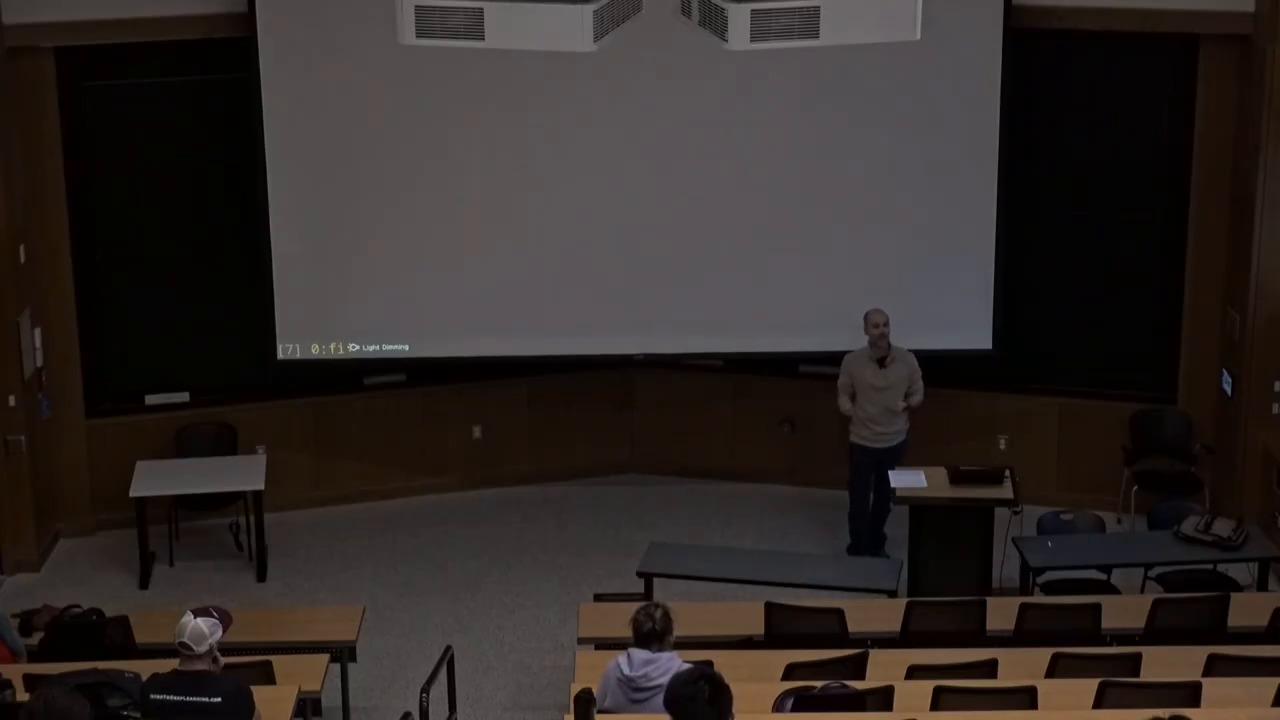
\includegraphics[width=0.92\textwidth]{figures/fig_01_room.jpg}
\caption{第四讲开场：讲者 Jon 在大屏幕前讲解调试的动机\vtag}
\end{figure}
\srcnote{00:05:00--00:05:15}
\end{minipage}


这一讲的主题是调试（debugging）与性能分析（profiling）。讲者 Jon 解释为什么需要调试：计算机是几乎无所不能的工具，但它们倾向于只做我们告诉它们的事，而这并不一定是我们想让它们做的事。调试就是去探索：我们想让计算机做什么，以及它根据我们的指令实际做了什么。

\subsection{打印调试}

讲者引用了 C 语言背后的名人之一 Brian Kernighan 的话：“最有效的调试工具仍然是仔细的思考，加上恰当放置的打印语句。”他说这对自己同样成立：他做的很多调试最终都是打印调试，也就是在代码里塞进一堆打印语句，输出有助于你思考程序在做什么的信息，找出你认为它应该做的和它实际做的在哪里不一致。打印调试被看作一种粗糙的“大棒”，但实际上在很多情况下非常好用。

\section{日志}

\subsection{从打印到日志}

打印调试最大的问题是每次都要从头开始：程序运行，你得开始缩小问题可能的来源。于是有了日志（logging）。讲者说，日志就是更有原则地使用打印语句：这些打印语句会长期留在代码里，而不只是为某一次调试临时加入；无论软件是坏了、你想了解它的性能，还是要实现一个功能，它们都能提供信息。所以在大型代码库、尤其是生产代码库中，你会看到大量日志。

日志可以是非结构化的，比如只是打印一段文字说明程序在做什么；也可以是结构化的，比如指标（metrics），甚至是随时间记录下来的 JSON 对象，便于在程序运行时更容易地从日志中提取信息。还记得第一讲的那些 Shell 工具吗？用它们来解析和提取日志中的信息往往很有用，而日志至少半结构化的话，事后用工具提取会容易得多。

\begin{knowledgebox}{日志级别}
日志有一些约定。通常每条日志至少有一个级别：trace、debug、info、warn、error、critical，表示这条日志有多重要。大多数应用和库都提供一种机制，只输出不低于某个级别的日志。比如在生产环境中关掉 trace 和 debug，只保留 info 及以上，或者只保留 warn 及以上，以免一直刷屏；调试时则打开更详细的日志。更成熟的日志框架还允许按模块、按文件设置：这部分应用用 trace 级别，其余部分只输出 warn，因为你只想深入这一部分。
\end{knowledgebox}

日志语句通常是主动加入的：写代码时你会想“这个大概值得记录”。而打印调试与日志之间的联系在于：当你做打印调试时，常常会意识到“这本应被记录下来，那我现在就不用临时打印了”。所以加完一堆打印语句之后，一个好的下一步是把它们改成日志语句。这样下一次程序正常运行时，你就能得到更多信息，更不需要经历修改、重新编译的循环来弄清程序的流程。

\subsection{第三方程序的日志}

你还会和很多第三方程序打交道，也许没有它们的代码，或者不知道怎么构建，至少构建起来很烦。很多第三方应用已经内置了日志，问题只是怎样访问。很多命令行工具可以传 \texttt{-v} 或 \texttt{-{}-verbose} 得到更多输出，而且这些参数常常可以叠加，比如 \texttt{-v -v} 或 \texttt{-vv}，表示更详细，可能让你看出程序在做什么、为什么表现得和预期不同。系统服务通常也能在操作系统里查看，比如 Linux 上一般用 \texttt{journalctl}，让它给出某个后台程序的全部输出，比如负责远程连接的 SSH 守护进程。

\section{调试器}

\subsection{GDB、LLDB 与 PDB}

讲者说，在写程序时，打印调试只能带你走这么远。到了一定阶段，要么每次重新编译、重新部署程序变得很烦，要么你根本不知道该记录什么，需要在程序执行时观察它，再决定提取什么信息，这时就要用调试器（debugger）。

最常见的是 GDB 和 LLDB。它们不是同一个程序，但界面和交互模型非常相似：附加到一个正在运行的进程上，让你控制它的执行。你可以让它在执行到代码的某一行时停下，在程序暂停时检查内存，让程序继续运行直到当前函数结束，诸如此类。它们是通用调试器，基本适用于任何程序，但更偏向编译过的原生程序，即用 C、C++、Rust 等语言写的、会在文件系统上生成二进制文件的程序。

对于其他语言，你通常想用特定语言的调试器。比如 Python 有 PDB，顾名思义它和 GDB 非常相似，但专门用于 Python 程序，交互方式相同：遇到某处时停下、监视某个变量并在它变化时通知你、检查程序状态等等。

\subsection{反向调试与 rr}

讲者接着介绍反向调试（reverse debugging），也叫记录回放调试。用调试器调试时，程序只是正常执行：从头开始，运行到退出，或者永远不退出；运行过程中你可以暂停和恢复，这是两种主要的控制手段。有时令人沮丧的是：你让程序运行，发现遇到了某个 bug，真正想做的是往回走，弄清是怎样到达这个 bug 的，比如是什么操作顺序让这个数变成 4 而不是 5，让这个布尔值变成 true 而不是 false。但那时程序早已越过了真正出错的地方。

反向调试对这类问题非常有用。Linux 上主要的工具之一叫 rr（record replay）。它的界面和 GDB 完全一样，所有命令都相同；唯一的区别是 rr 会记录程序所做的一切，包括它与操作系统、与内存的所有交互，全部写下来，使程序能够反向执行。用 rr 启动程序时，它从头到尾运行程序并记录发生的一切。这样当你停在某个断点时，就可以反向单步：不是执行下一行，而是撤销当前这一行，假装回到程序上一行的世界，并检查那时的状态。讲者说这在追踪棘手的 bug 时非常强大。

\begin{warningbox}{海森堡 bug}
讲者提到一类 bug 叫海森堡 bug（Heisenbug），名字来自不确定性原理：你试图观察它时，它就消失了。打印调试时最常遇到：打印会拖慢程序，因为程序要停下来往终端写一堆字符再继续运行，这点小小的延迟有时就会让程序的行为与全速运行时不同，并发程序尤其如此，bug 可能正是因为一个线程比另一个快才出现。调试器也会改变程序的执行方式，rr 尤其明显：为了记录完整的执行过程，它使用确定性调度器，以非常特定的顺序运行所有线程，而你的 bug 可能在这种顺序下根本不出现。所以有时选择工具不仅要看它提供什么能力，还要看能不能在它里面复现问题。
\end{warningbox}

\subsection{演示：被篡改的账户 ID}

\noindent\begin{minipage}{\textwidth}
\begin{figure}[H]
\centering
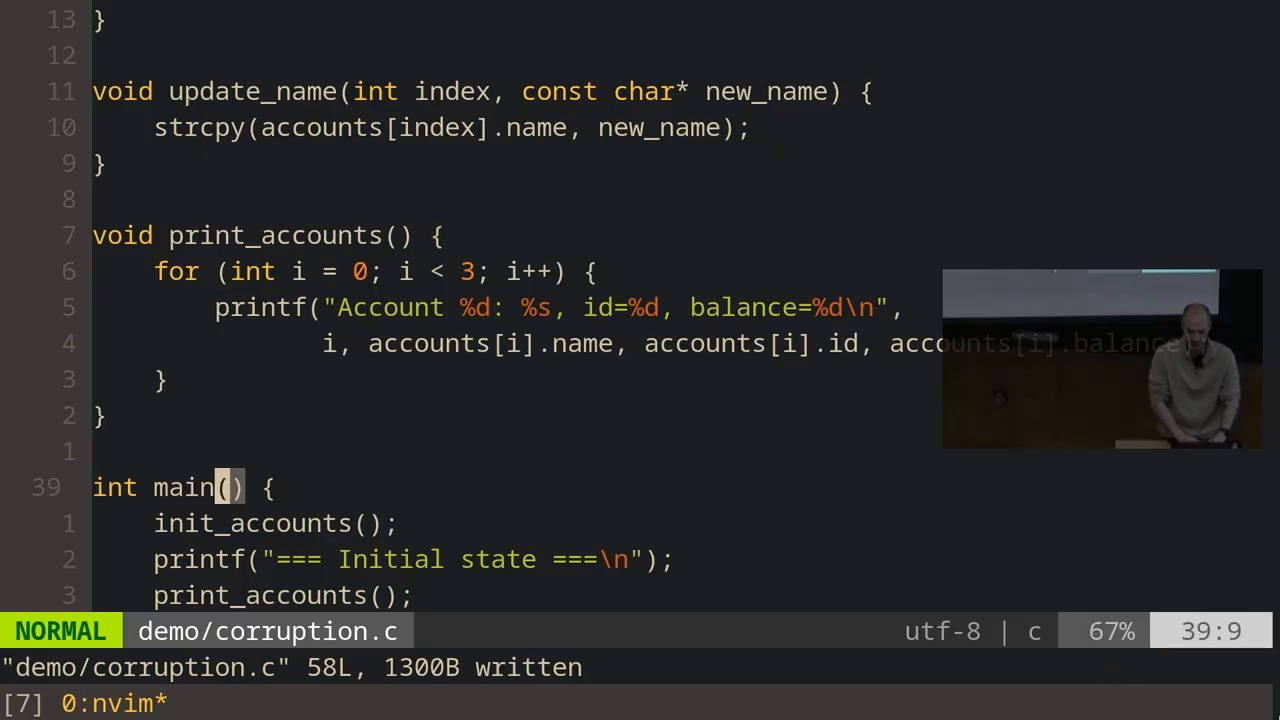
\includegraphics[width=0.92\textwidth]{figures/fig_02_corruption_src.jpg}
\caption{corruption.c：Account 结构体、update\_name 与 print\_accounts 函数\vtag}
\end{figure}
\srcnote{00:12:00--00:12:15}
\end{minipage}


讲者展示了一个 C 程序 \texttt{corruption.c}，它也出现在习题里。程序中有一个结构体，包含一个字符串类型的名字、一个 ID 和一个余额；有 Alice、Bob、Charlie 三个账户，各有一定金额。有一个函数可以修改账户的名字，另一个打印所有账户的余额。程序先打印账户的初始状态，然后修改一些余额。讲者说他已经把 bug 缩小了一些：修改余额和名字之后打印账户时，某个账户的 ID 变了。初始设置中账户 0 的 ID 是 1，账户 1 是 2，账户 2 是 3，可上面的代码没有改过任何 ID，只改了余额和名字字段，为什么 ID 错了？

\noindent\begin{minipage}{\textwidth}
\begin{figure}[H]
\centering
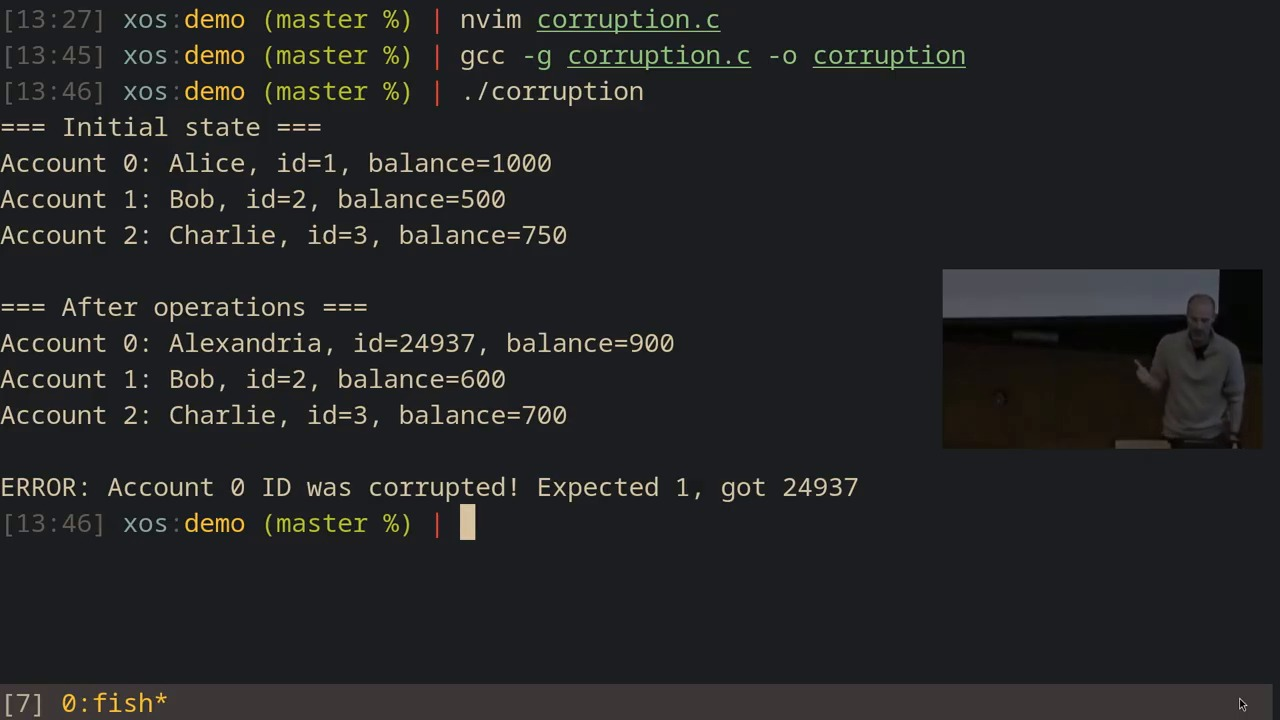
\includegraphics[width=0.92\textwidth]{figures/fig_03_compile_run.jpg}
\caption{用 \texttt{gcc -g} 编译后运行：Alexandria 的名字正确，但 ID 变成了奇怪的数字\vtag}
\end{figure}
\srcnote{00:13:45--00:14:00}
\end{minipage}


他先编译程序：\texttt{gcc -g corruption.c -o corruption}。\texttt{-g} 表示包含调试符号，也就是在程序里保留变量名、函数名等信息，这样之后在调试器里打开时，看到的不只是内存地址和二进制数据，而是知道“这些汇编指令其实是源代码中的这个函数”，它保留了这种映射；\texttt{-o} 指定编译结果放在哪里。运行后，初始状态如预期；但操作之后，账户 0 的名字正确地变成了 Alexandria，ID 却是一个完全不同的数字。

\noindent\begin{minipage}{\textwidth}
\begin{figure}[H]
\centering
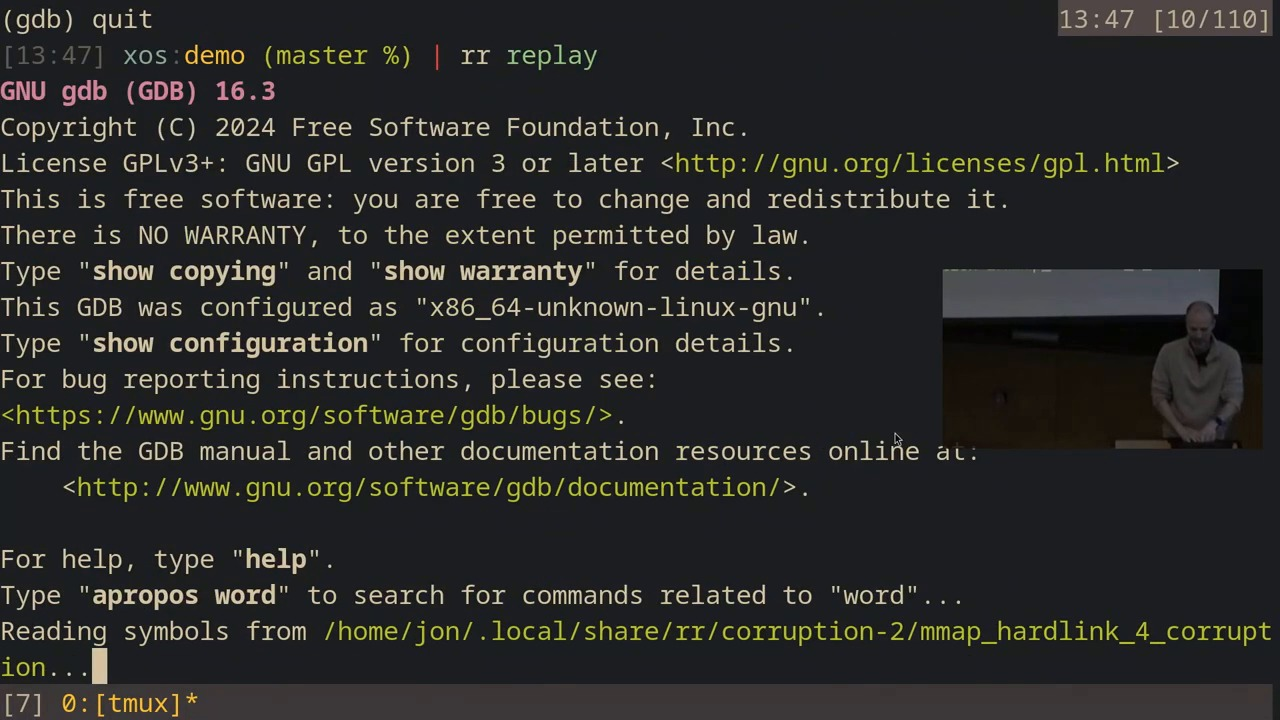
\includegraphics[width=0.92\textwidth]{figures/fig_04_rr_replay.jpg}
\caption{\texttt{rr replay} 打开的界面就是 GDB\vtag}
\end{figure}
\srcnote{00:15:00--00:15:15}
\end{minipage}


接下来用 \texttt{rr record ./corruption} 记录执行过程：它运行程序，记录它所做的一切，存到磁盘上的文件里（在隐藏目录中，所以看不到）。然后 \texttt{rr replay} 加载这个文件，恢复运行这个程序的会话。讲者对比了直接用 GDB：没有记录和回放，只是运行程序，留下一个可以操作的提示符；而 \texttt{rr replay} 看起来几乎一样，仔细看它打印的确实是 GDB。程序停在开头，输入 continue，它运行程序，打印出和正常运行时一样的内容。如果程序崩溃，它会停在崩溃处；但这个程序不崩溃，只是打印一条“这个 ID 看起来不对”的消息。

\begin{lstlisting}[language=bash]
gcc -g corruption.c -o corruption
./corruption
rr record ./corruption
rr replay
\end{lstlisting}

\subsection{断点与查看状态}

\noindent\begin{minipage}{\textwidth}
\begin{figure}[H]
\centering
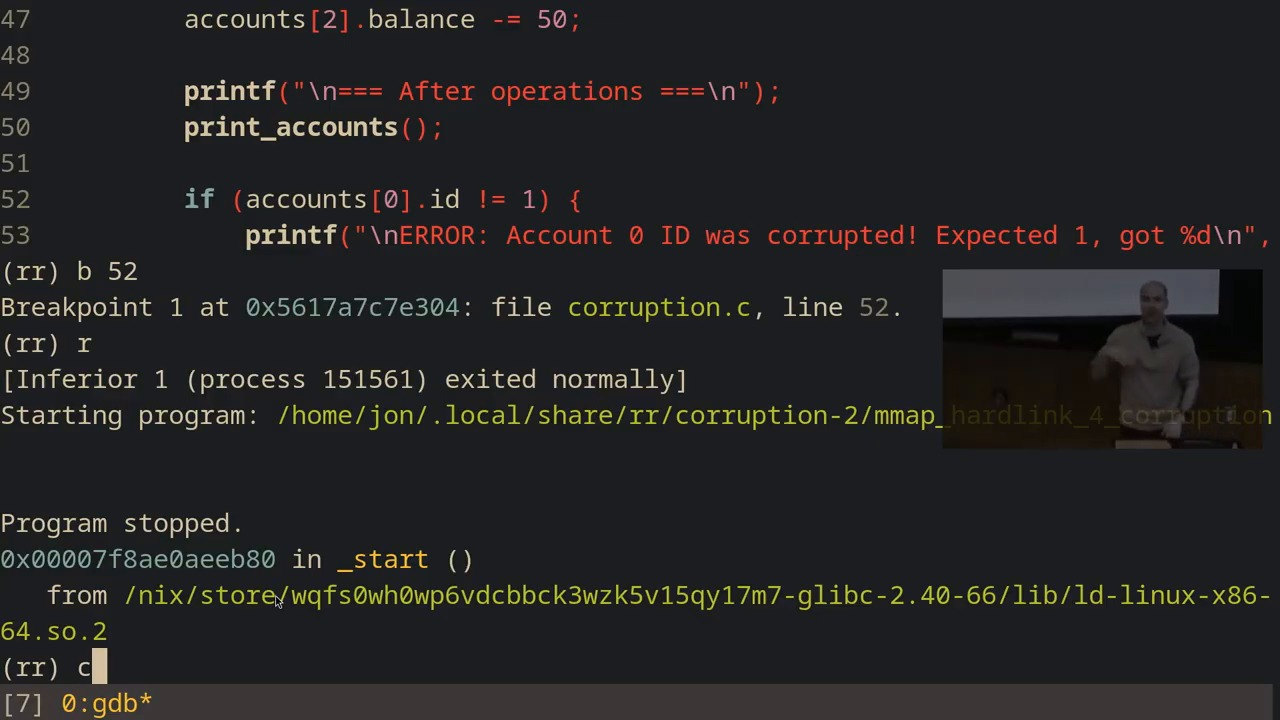
\includegraphics[width=0.92\textwidth]{figures/fig_05_breakpoint.jpg}
\caption{在第 52 行设断点，用 r 重新开始、c 继续，程序停在检查 ID 的 if 语句处\vtag}
\end{figure}
\srcnote{00:16:30--00:16:45}
\end{minipage}


要弄清为什么会进入那个 if 条件，可以输入 \texttt{list}，它打印出 GDB（或 rr）看到的源代码，再输入 \texttt{list} 可以列出更多行。他想在下面这个 if 上设断点：当执行到这一行，也就是二进制中对应这部分时，停止执行并把控制权交给他。于是输入 \texttt{break 52}，然后 \texttt{r}（run）从头开始程序，因为刚才已经运行结束了；再按 \texttt{c}（continue），因为 \texttt{r} 只是把程序放到开头，还不让它运行，好让你设断点。此时程序计数器（指示我们在二进制中位置的东西）指向 \texttt{main} 函数的开头；继续之后，它执行 \texttt{main}，一直到遇到第一个断点。

现在可以检查程序状态，比如用 \texttt{p}（print，也可以写全）打印 \texttt{accounts[0].id}。在这个作用域里可以访问函数中的任何局部变量，相当于注入几行立即执行并打印结果的代码。还有许多变化：可以用十六进制打印，可以这样浏览结构体和数组，甚至可以在这里调用函数。讲者说这是一个相当丰富的环境，不会全部讲。

\subsection{监视点与反向继续}

\noindent\begin{minipage}{\textwidth}
\begin{figure}[H]
\centering
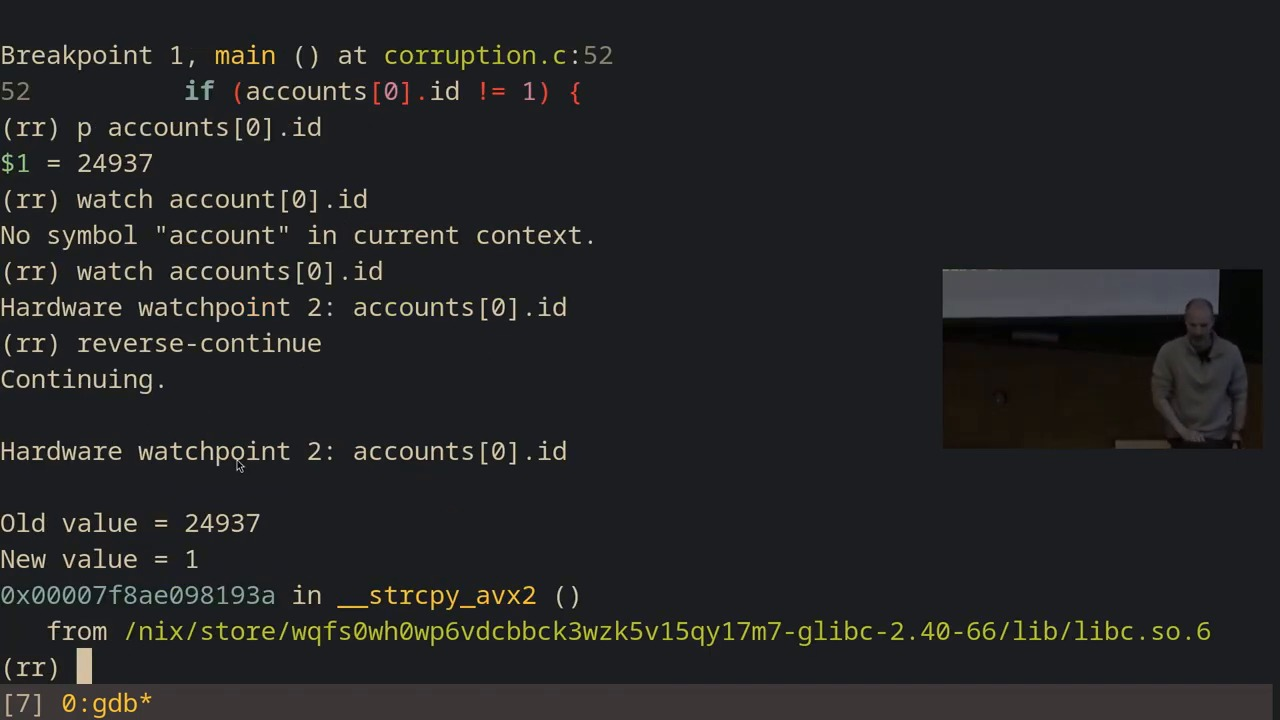
\includegraphics[width=0.92\textwidth]{figures/fig_06_watch_reverse.jpg}
\caption{设置 watch 后执行 reverse-continue，停在 ID 从 1 被改写的那一刻\vtag}
\end{figure}
\srcnote{00:19:00--00:19:15}
\end{minipage}


他真正想知道的是：ID 是什么时候变的，什么时候从 1 变成这个怪数？用 GDB 就没办法了，因为此时它已经被篡改了，只能继续运行到程序结束。他得把断点设得越来越早，一次又一次地运行，看到“在这里设断点时还没被篡改”，然后自己去搜索。用 rr 可以做件很酷的事：\texttt{watch accounts[0].id}，即监视这个表达式，值一变就中断，这在 GDB 里也能做；但在 rr 里还可以 \texttt{reverse-continue}：不是继续往下执行，而是撤销 \texttt{main} 中已执行的行，直到这个值发生变化。

反向继续后，它报告命中了这个表达式的硬件监视点：旧值是那个怪数，新值是 1。讲者提醒，因为是反向执行，从未来往回走，“新值”其实是较早的值，“旧值”是较新的值。这里就是值改变的地方。接着用 \texttt{bt}（backtrace）查看调用栈，它列出到当前行为止的整条函数调用链：实际修改 ID 的函数是 C 库中的某个 \texttt{\_\_strcpy\_avx2}，调用它的是 \texttt{update\_name}，下面还能看到出问题时传给它的参数：传入新名字 Alexandria，调用 \texttt{update\_name}，执行字符串复制，结果不知为何改了 ID。

\noindent\begin{minipage}{\textwidth}
\begin{figure}[H]
\centering
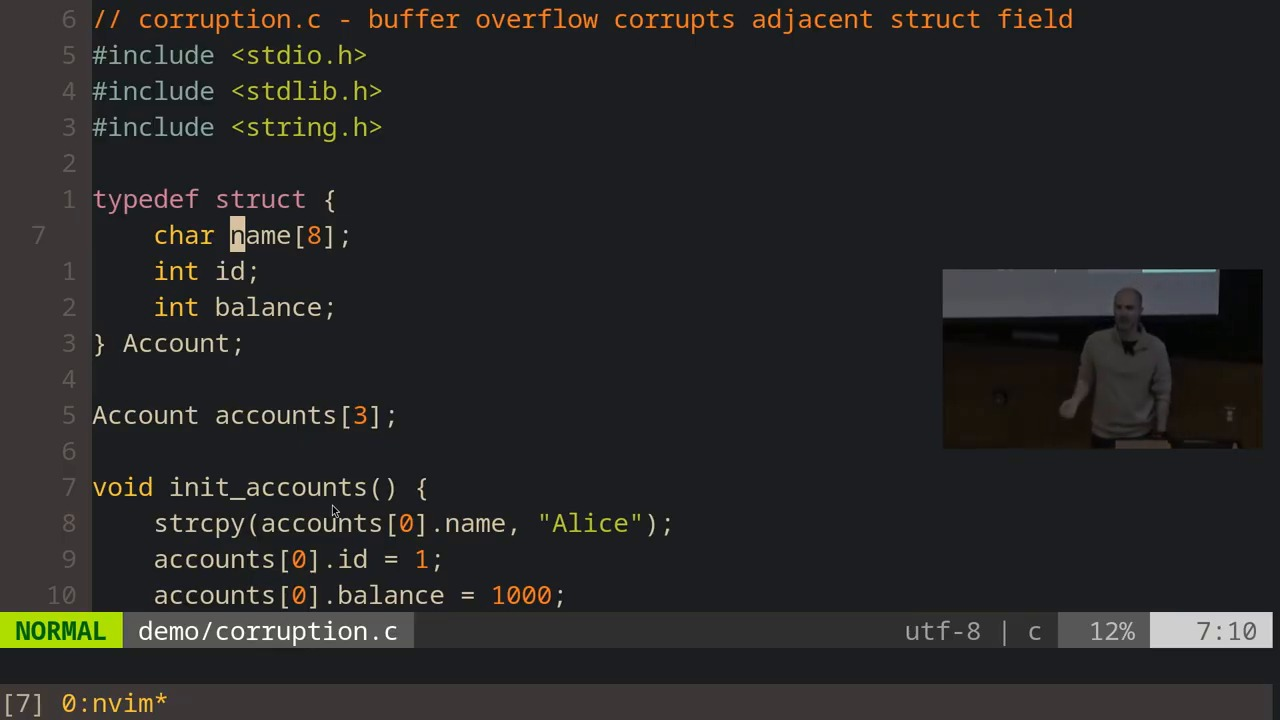
\includegraphics[width=0.92\textwidth]{figures/fig_07_struct_name8.jpg}
\caption{结构体中 name 只有 8 个字节，紧随其后的字段就是 id\vtag}
\end{figure}
\srcnote{00:21:00--00:21:15}
\end{minipage}


这立刻告诉我们问题出在哪个函数。\texttt{list update\_name} 显示这个函数只做了一件事：字符串复制，复制到 \texttt{accounts[index].name}。那不是 ID，为什么会出问题？回到结构体定义，\texttt{name} 只有 8 个字节长；Alexandria 加上作为字符串结束符的空字节，超过了 8 个字符。于是复制写过了这个字段的末尾，而下一个字段就是 ID，字符串复制把 ID 覆盖了。

\begin{lstlisting}[language=bash]
(rr) break 52
(rr) run
(rr) continue
(rr) print accounts[0].id
(rr) watch accounts[0].id
(rr) reverse-continue
(rr) bt
(rr) list update_name
\end{lstlisting}

\begin{importantbox}{rr 的价值}
讲者总结：调试器能轻松做这种事，而 rr 让它更容易，因为你不必事先知道要停在哪里，可以往回走。rr 尤其适合偶发失败的测试和难以复现的崩溃：第一讲那个循环运行测试直到失败的脚本，如果把写日志改成 \texttt{rr record}，就会一直录制直到失败，然后 \texttt{rr replay} 就得到一次可以前后反复穿梭的失败执行。
\end{importantbox}

\begin{knowledgebox}{GDB 常用命令}
讲义作者整理：\texttt{break 文件:行号} 或 \texttt{break 函数名} 设断点；\texttt{run} 从头运行；\texttt{continue} 继续；\texttt{next} 执行下一行（不进入函数）；\texttt{step} 进入函数；\texttt{finish} 运行到当前函数返回；\texttt{print 表达式} 打印值（\texttt{p/x} 以十六进制）；\texttt{watch 表达式} 设置监视点；\texttt{bt} 打印调用栈；\texttt{list} 显示源码；\texttt{quit} 退出。rr 额外提供 \texttt{reverse-next}、\texttt{reverse-step}、\texttt{reverse-continue} 等反向命令。
\end{knowledgebox}

\subsection{rr 的局限与 GDB 的重新运行}

rr 并不总能用：它在虚拟机上效果不好，因为需要硬件支持，要能监视 CPU 中的某些东西才能记录；它也只支持 Linux。GDB 和 rr 共同的问题是，修改程序之后必须退出会话、重新编译，再打开 GDB；对 rr 来说录制也失效了，因为那是旧二进制的录制，无法用于新版本。

\noindent\begin{minipage}{\textwidth}
\begin{figure}[H]
\centering
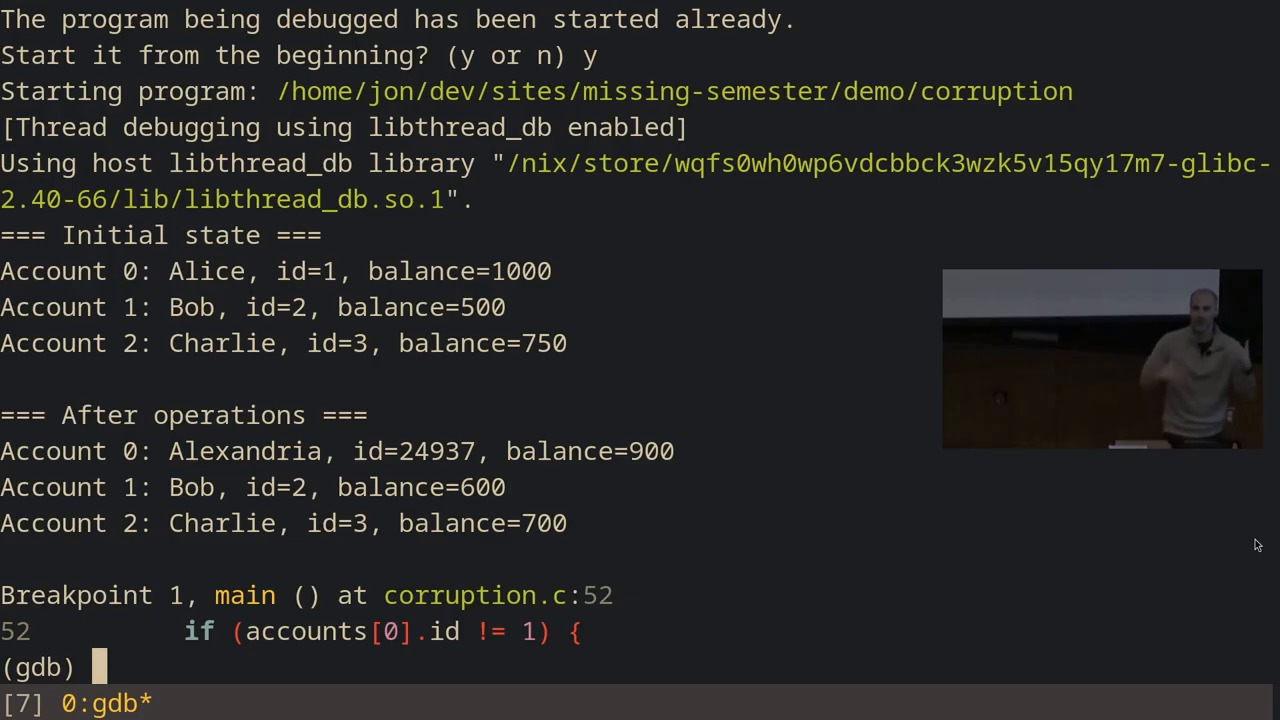
\includegraphics[width=0.92\textwidth]{figures/fig_08_gdb_rerun.jpg}
\caption{在 GDB 中再次输入 run 会从头开始，并保留已设置的断点\vtag}
\end{figure}
\srcnote{00:24:00--00:24:15}
\end{minipage}


有同学问能否方便地重新运行。讲者演示：\texttt{gdb corruption}，在 51 行设断点，\texttt{run}，程序停住；用 \texttt{next} 执行下一条语句，再 \texttt{next} 往下走。想从头开始，就再输入 \texttt{run}，它从头启动程序，但保留所有断点。这就是在 GDB 里二分查找的方式。也可以 \texttt{watch accounts[0].id} 再从头运行，它会告诉你这个字段第一次被修改的位置，继续则停在下一次修改，同样指向这个 bug。

\section{追踪}

\subsection{strace：系统调用追踪}

讲者说，有时 bug 并不在你的代码里，或者你只是想了解程序在做什么、卡在什么上，不关心代码，那是别人的代码。你只想知道它在做什么、为什么失败、CPU 周期花在哪里。这时就需要追踪（tracing），追踪一个已有的进程。最常见的机制之一是 \texttt{strace}，它追踪一个进程发出的系统调用：可以是 \texttt{strace} 加程序名启动的进程，也可以是 \texttt{strace -p} 加进程 ID，附加到一个已在运行的程序上。

\noindent\begin{minipage}{\textwidth}
\begin{figure}[H]
\centering
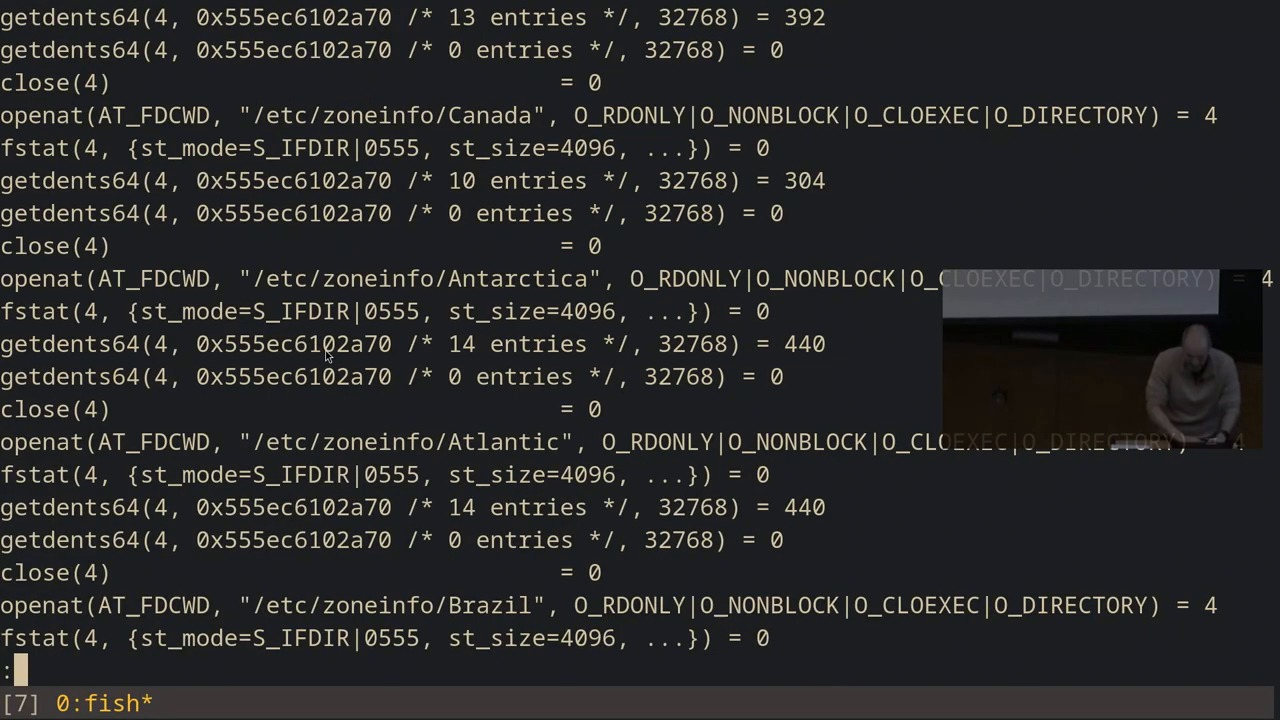
\includegraphics[width=0.92\textwidth]{figures/fig_09_strace_raw.jpg}
\caption{\texttt{strace ls -l} 的输出：每行一个系统调用，包括读取时区文件\vtag}
\end{figure}
\srcnote{00:28:00--00:28:15}
\end{minipage}


讲者运行 \texttt{strace ls -l /tmp}，用 \texttt{2>\&1} 这个 bash 重定向技巧把错误和标准输出都送到同一处，再通过管道交给分页器 \texttt{less}，这样输出不会倾倒在终端里，而是打开一个可以上下滚动的小程序，输出很多时这很有用。得到的是一长串行，仔细看会发现每行都以一个函数名和左括号开头，后面是参数列表。这些就是程序发出的所有系统调用。系统调用是你请求操作系统、请求内核做的事：启动或停止进程、打开文件、读文件、写东西、访问网络套接字等等；它们不是你程序内部的函数。

开头的那些是启动一个进程所需的：告诉操作系统执行磁盘上的这个文件，加载它可能依赖的共享库，所以对我们来说没多大意思。往下滚动，可以看到它打开了一堆时区文件：因为要求长格式输出，它要打印文件的修改时间，就需要时区信息来换算成本地时间。

\subsection{过滤与跟踪子进程}

\noindent\begin{minipage}{\textwidth}
\begin{figure}[H]
\centering
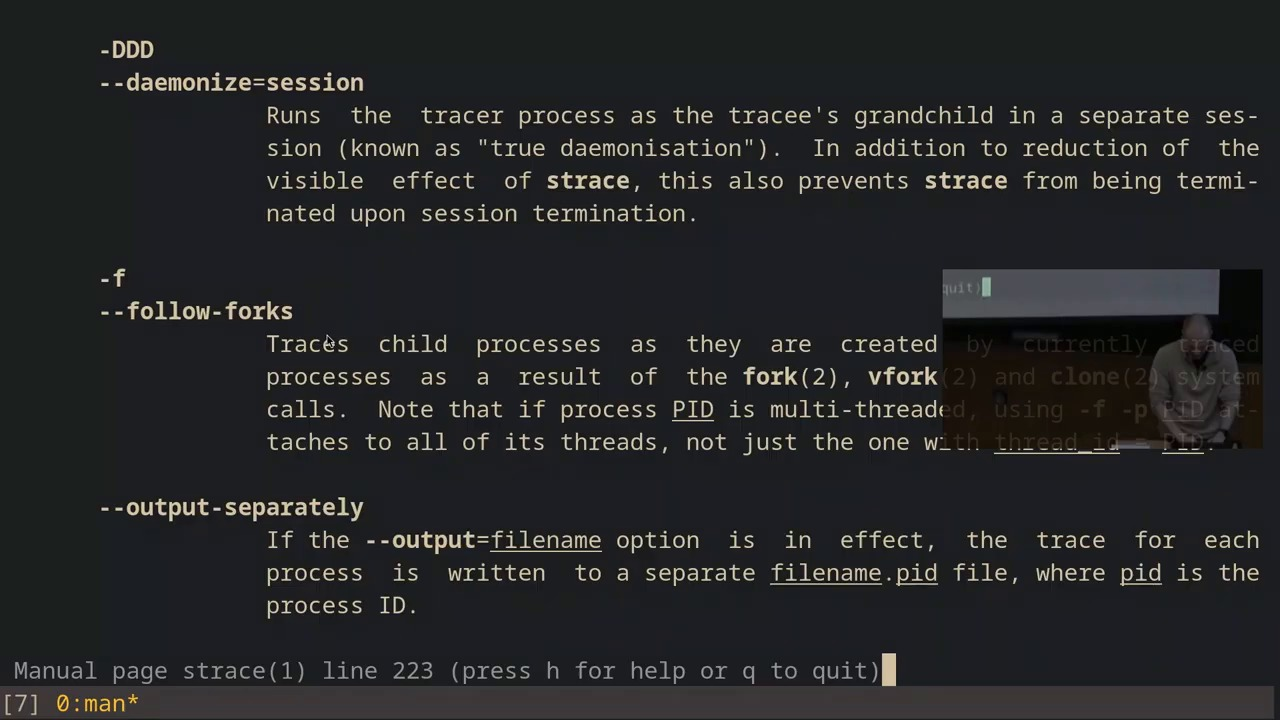
\includegraphics[width=0.92\textwidth]{figures/fig_10_strace_man.jpg}
\caption{strace 手册中关于 -f（\texttt{-{}-follow-forks}）的说明\vtag}
\end{figure}
\srcnote{00:31:00--00:31:15}
\end{minipage}


输出太多，很难找到想要的东西。可以只显示某类操作相关的调用，比如 \texttt{-e trace=\%file} 只显示与文件相关的，网络、加载动态库等就不列了；还可以缩小到某个特定的系统调用。讲者想看 \texttt{getdents} 之类读取目录的调用，却什么都没看到。他意识到原因在于 Nix：\texttt{strace} 运行你给它的程序，而如果那个程序又启动了别的程序，默认不会追踪它们。在 Nix 上，\texttt{ls} 实际上是一个包装程序，它再调用真正的 \texttt{ls}。翻看手册，\texttt{strace} 有一个 \texttt{-f}（\texttt{-{}-follow-forks}）参数，表示也追踪它启动的其他命令。

\noindent\begin{minipage}{\textwidth}
\begin{figure}[H]
\centering
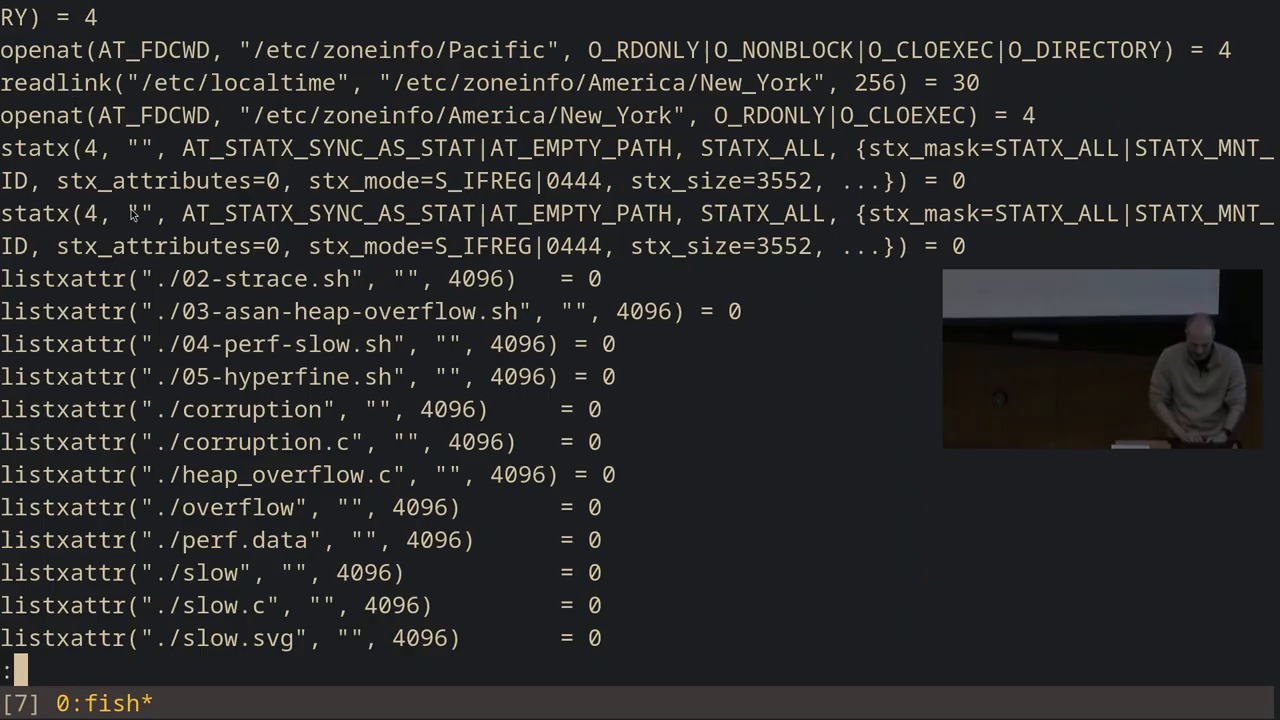
\includegraphics[width=0.92\textwidth]{figures/fig_11_strace_f.jpg}
\caption{加上 -f 后，长格式输出对每个目录项都调用 listxattr 和 statx\vtag}
\end{figure}
\srcnote{00:33:00--00:33:15}
\end{minipage}


加上 \texttt{-f} 后，可以看到程序用来打开当前目录的那一行：以目录方式打开“.”，供后面读取目录项。因为传了 \texttt{-l}，要求给出每个文件的更多信息，它还对目录中的每一项调用 \texttt{listxattr} 和 \texttt{statx}，因为不只要列出名字，还要收集额外信息。这说明传 \texttt{-l} 时 \texttt{ls} 做了更多工作。讲者说，用 \texttt{-p} 附加到正在运行的进程上时，它会打印大量关于进程在做什么的信息；如果什么都不打印，说明那个进程只是在做 CPU 计算，根本没在和操作系统交互。\texttt{man strace} 的过滤部分列出了可以过滤的各类调用：某个具体系统调用，\texttt{all}（默认），\texttt{\%file}，以及进程相关、网络相关等。

\begin{lstlisting}[language=bash]
strace ls -l /tmp 2>&1 | less
strace -f -e trace=%file ls -l 2>&1 | less
strace -f -e trace=statx ls -l
strace -p 1234
\end{lstlisting}

\begin{practicebox}{用 strace 观察程序}
讲义作者整理：分别运行 \texttt{strace -c ls} 和 \texttt{strace -c ls -l}，\texttt{-c} 会在结束时给出每种系统调用的次数统计，比较两者的差别，验证讲者关于 \texttt{-l} 需要额外 \texttt{statx} 调用的说法；再用 \texttt{strace -f -e trace=\%network curl https://example.com} 观察一次网络请求涉及哪些系统调用。
\end{practicebox}

\subsection{eBPF 与 bpftrace}

\noindent\begin{minipage}{\textwidth}
\begin{figure}[H]
\centering
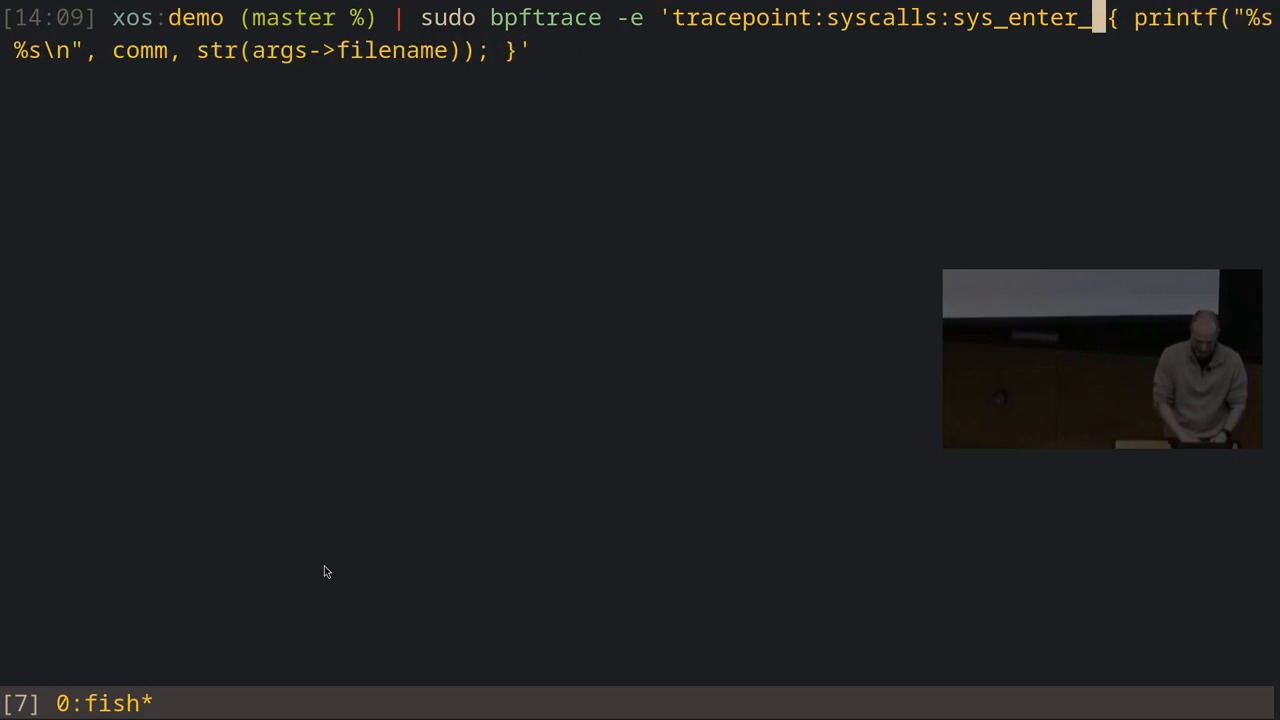
\includegraphics[width=0.92\textwidth]{figures/fig_12_bpftrace_count.jpg}
\caption{bpftrace 的第一个尝试：在每个 sys\_enter 探针上计数\vtag}
\end{figure}
\srcnote{00:38:00--00:38:15}
\end{minipage}


讲者说 \texttt{strace} 只做系统调用追踪。如果想做更花哨的事呢？比如统计内核中读取调用耗时的分布图，\texttt{strace} 只告诉你这个函数用这些参数被调用了。你真正需要的是能把程序几乎注入到内核里去测量想测的东西，这也存在，叫 eBPF（扩展伯克利包过滤器）：一些可以安装到 Linux 内核中、以内核权限运行的小程序。可以用 C 写，表达能力极强，但也有更方便的用户工具，比如 \texttt{bpftrace}，它像 \texttt{strace}，但用的是 eBPF，并允许写更高级的表达式。

\texttt{bpftrace} 接受 \texttt{-e} 参数，后面是一个表达式，说明执行什么、何时执行。讲者说这些表达式像第一讲简要提过的 \texttt{awk} 表达式：可以按系统调用过滤，按参数过滤，并说明这个调用发生时做什么，语言有点古怪，但相当灵活。第一个例子是追踪所有进入系统调用的追踪点：\texttt{sys\_enter} 是内核对“程序开始一个系统调用”的称呼，星号是一个模式，也可以换成比如 \texttt{statx}。花括号里是一小段 BPF 程序，可以写 C，也有一些便捷语法：\texttt{@} 是一个映射，\texttt{probe} 表示被追踪对象的名字（这里就是系统调用名），\texttt{count()} 每调用一次加一，于是统计每个系统调用的调用次数。运行后没有输出，直到结束进程时才打印出整个映射。讲者这次运行遇到了报错，他推测因为 \texttt{bpftrace} 默认追踪整个内核，不只是某个程序，而是电脑上正在发生的一切。

\noindent\begin{minipage}{\textwidth}
\begin{figure}[H]
\centering
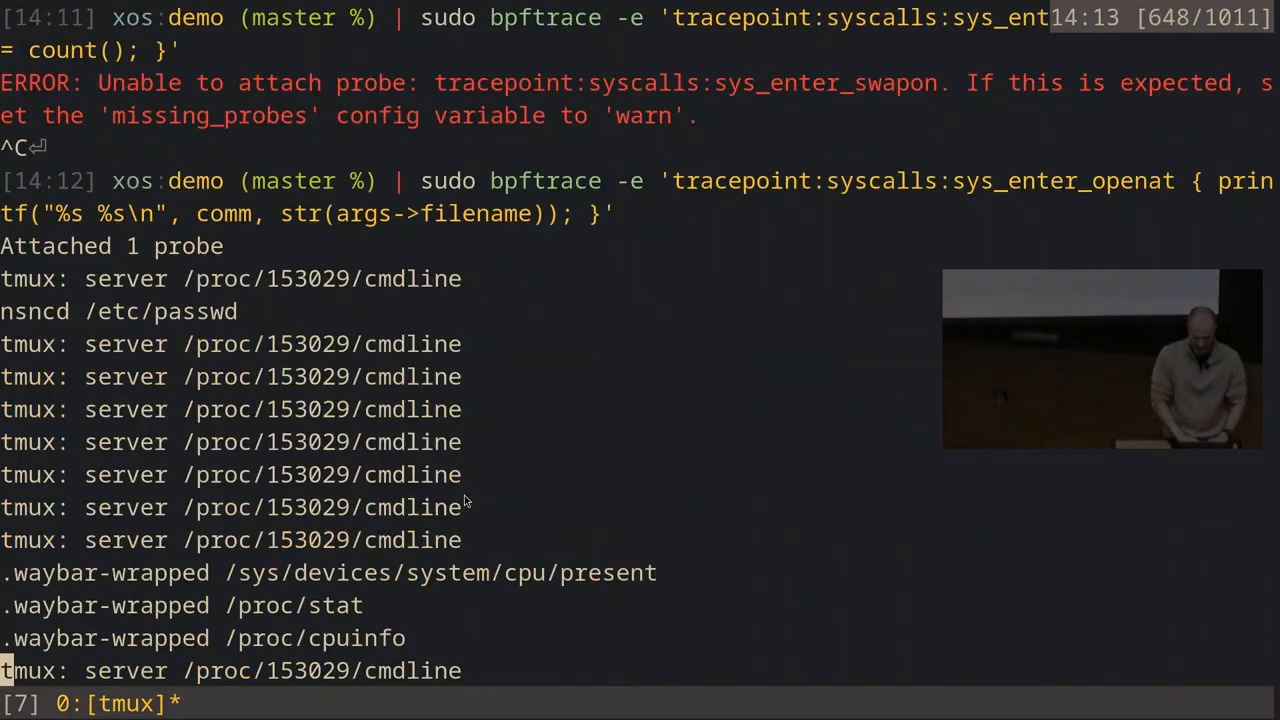
\includegraphics[width=0.92\textwidth]{figures/fig_13_bpftrace_openat.jpg}
\caption{追踪 openat：实时打印电脑上每个程序打开的每个文件\vtag}
\end{figure}
\srcnote{00:41:00--00:41:15}
\end{minipage}


于是他换了一个稍复杂的：追踪所有 \texttt{openat} 系统调用，打印 \texttt{comm}（执行操作的程序名）和作为文件名的字符串参数，也就是打印每一个被打开的文件。运行后它附加探针，持续打印电脑上任何程序打开任何文件的信息。还可以加限制，比如只追踪 \texttt{comm} 等于 tmux 的调用。

\noindent\begin{minipage}{\textwidth}
\begin{figure}[H]
\centering
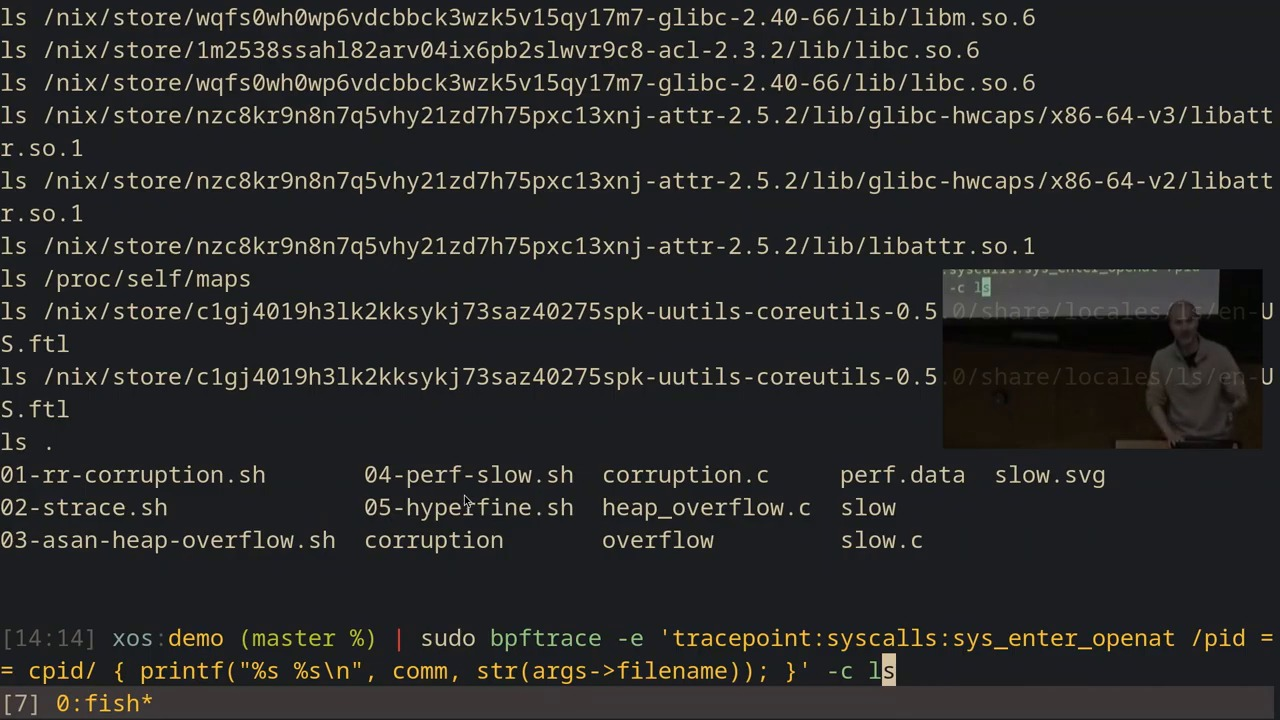
\includegraphics[width=0.92\textwidth]{figures/fig_14_bpf_cpid.jpg}
\caption{用 \texttt{-c ls} 启动命令，并用 pid == cpid 只追踪它的 openat\vtag}
\end{figure}
\srcnote{00:42:00--00:42:15}
\end{minipage}


另一个方便的写法：要求进程 ID 等于 \texttt{cpid}，再传 \texttt{-c ls}。\texttt{-c} 表示运行后面的命令，并把特殊变量 \texttt{cpid} 设为刚启动进程的 ID，这样就只追踪你运行的程序的 \texttt{openat} 调用。

\begin{lstlisting}[language=bash]
sudo bpftrace -e 'tracepoint:syscalls:sys_enter_* { @[probe] = count(); }'
sudo bpftrace -e 'tracepoint:syscalls:sys_enter_openat
  { printf("%s %s\n", comm, str(args->filename)); }'
sudo bpftrace -e 'tracepoint:syscalls:sys_enter_openat /pid == cpid/
  { printf("%s %s\n", comm, str(args->filename)); }' -c ls
\end{lstlisting}

\noindent\begin{minipage}{\textwidth}
\begin{figure}[H]
\centering
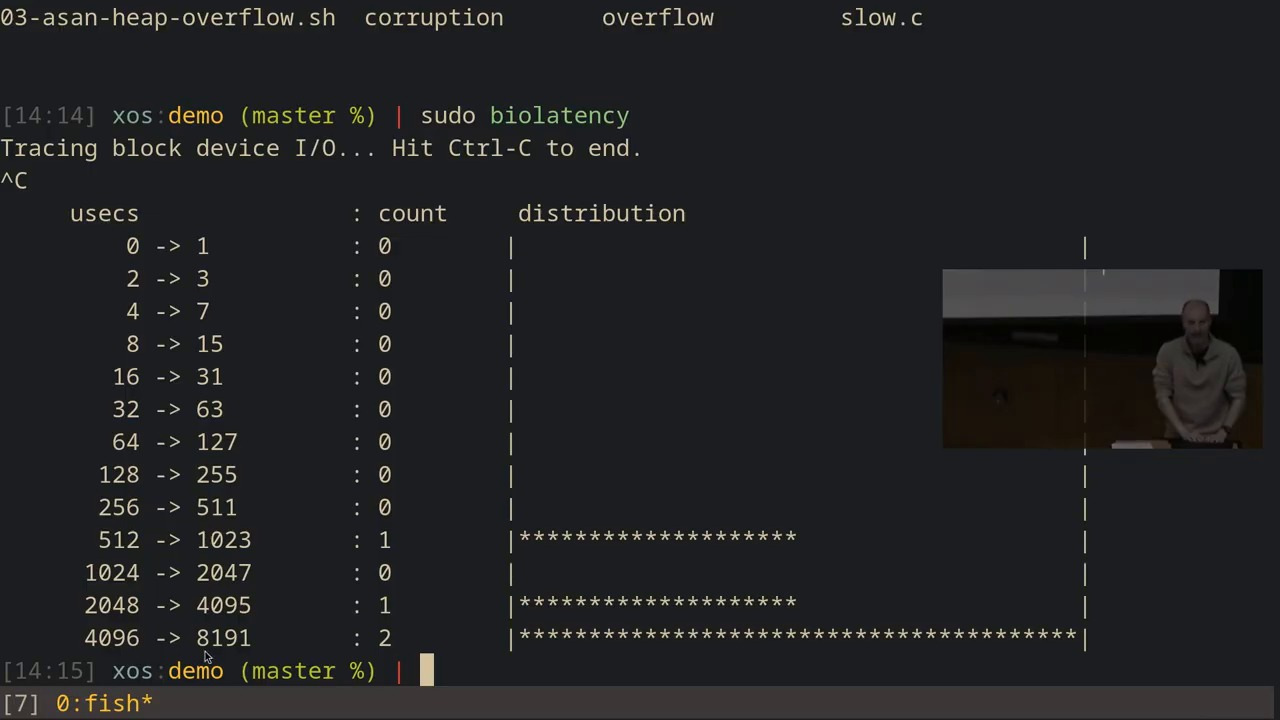
\includegraphics[width=0.92\textwidth]{figures/fig_15_biolatency.jpg}
\caption{biolatency 以直方图显示磁盘 I/O 耗时的分布\vtag}
\end{figure}
\srcnote{00:43:00--00:43:15}
\end{minipage}


讲者说，有了这些就能做很花哨的事，好在很多人已经替我们写好了。比如 \texttt{biolatency}，它完全用 BPF 写成，监视所有磁盘操作，测量从开始到结束花了多久，也就是监视每个涉及磁盘的调用的进入和退出，然后以直方图显示：有两个花了 4 到 8 微秒，一个花了 2 到 4 微秒，等等，运行越久收集的数据越多。还有 \texttt{opensnoop}，基本就是刚才那个程序：窥探电脑上每一次打开调用，任何程序打开任何文件时，打印出进程和它打开的东西。这些都由 BPF 基础设施实现，可以用来追踪程序几乎做的任何事，对弄清程序在做什么、为什么卡住非常有用。

\subsection{tcpdump 与网络调试}

\noindent\begin{minipage}{\textwidth}
\begin{figure}[H]
\centering
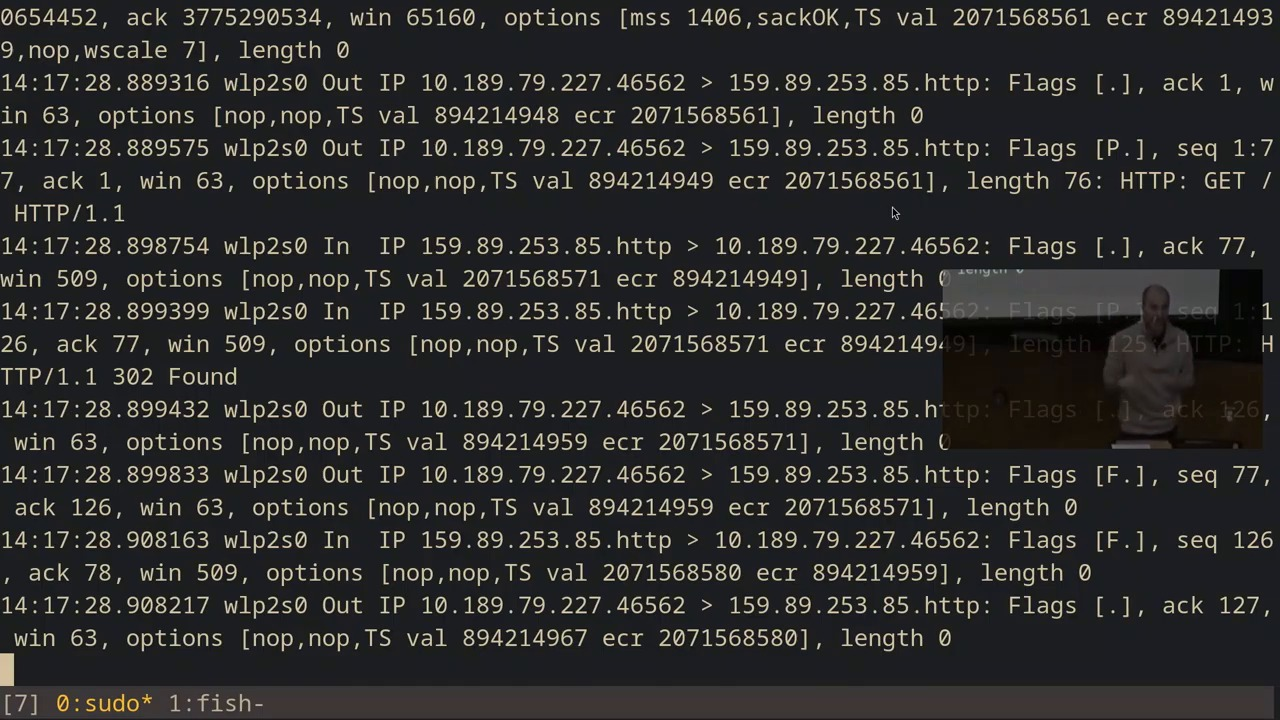
\includegraphics[width=0.92\textwidth]{figures/fig_16_tcpdump.jpg}
\caption{tcpdump 抓取发往 80 端口的数据包，每行列出地址、端口、标志和长度\vtag}
\end{figure}
\srcnote{00:45:00--00:45:15}
\end{minipage}


还有别的东西可以追踪，比如网络。\texttt{tcpdump} 会导出经过网络接口的流量。讲者的无线网卡接口名叫 \texttt{wlp2s0}，也可以写 \texttt{any} 表示所有接口；然后写一个 tcpdump 表达式，说明要记录哪类网络数据包，比如发往 80 端口的所有包。一开始没有包，他在另一个终端用 \texttt{curl} 访问一个只支持 HTTP 的网站（neverssl.com），回到 tcpdump，就看到一批发往 HTTP 端口的包。之所以有一批，是因为它不记录单个请求，而是记录经过接口发往 80 端口的每个包：消息很短，但一个 HTTP 请求需要多个 IP 包，响应也一样。每个包都打印出源 IP、目的 IP、源端口、目的端口、IP 标志、TCP 窗口信息、选项、包长度等。

讲者说这在调试网络协议时非常有用，因为可以记录关于包的任何信息，包括内容；Wireshark 之类的工具还理解建立在 IP 之上的各种协议，比如有一个理解 MySQL 的插件，接到网络接口上就能显示所有 MySQL 流量和包的内容；你也可以为自己设计的协议写插件，在包的层面调试协议。还可以录下数据包供以后回放，用于离线测试。它对加密流量会很吃力，因为记录的是原始 IP 包；但有 mitmproxy（中间人代理）这样的工具，它假装是 HTTPS 服务器，解密后把包记录到磁盘。

\begin{lstlisting}[language=bash]
sudo tcpdump -i any port 80
curl http://neverssl.com
\end{lstlisting}

\section{自动化检查：Sanitizer 与 Valgrind}

\subsection{AddressSanitizer}

\noindent\begin{minipage}{\textwidth}
\begin{figure}[H]
\centering
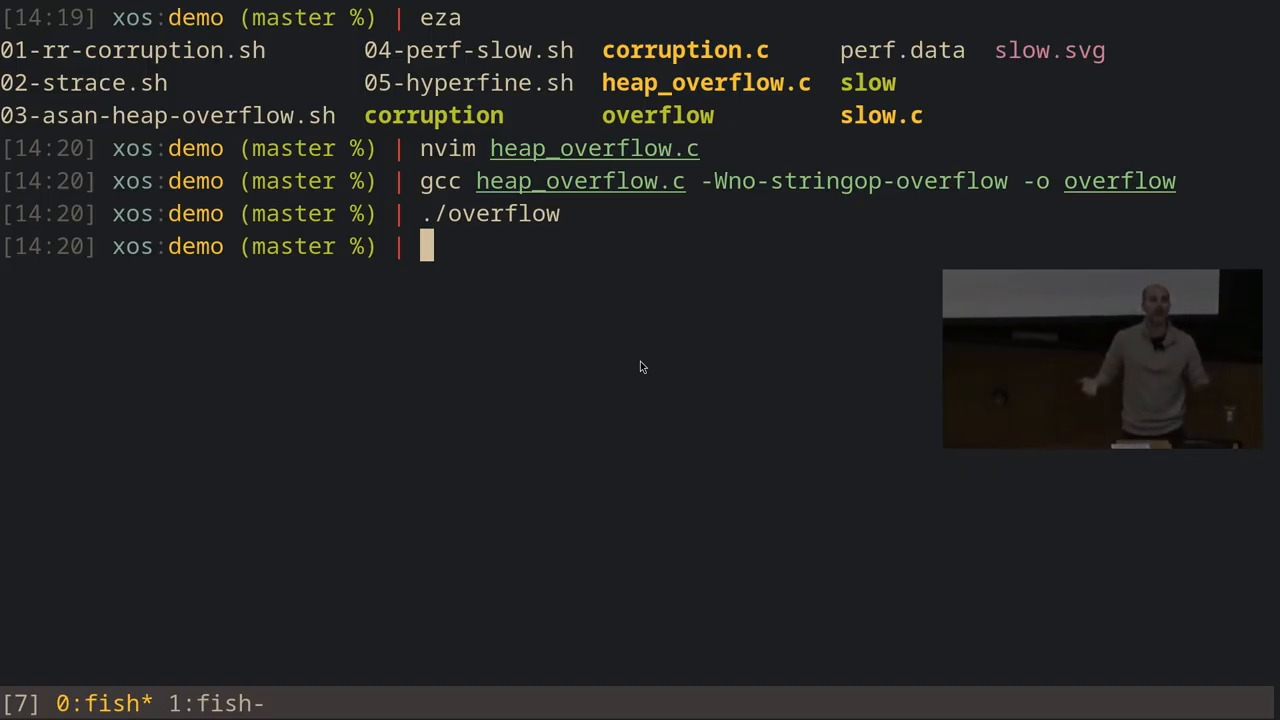
\includegraphics[width=0.92\textwidth]{figures/fig_17_heap_overflow.jpg}
\caption{heap\_overflow.c 正常编译运行时毫无异常，再加上 -fsanitize=address 重新编译\vtag}
\end{figure}
\srcnote{00:48:00--00:48:15}
\end{minipage}


讲者说，不是所有调试都必须手动，有时可以让程序替你做。近来最常见的之一是 sanitizer：编译器的小扩展，让编译器在程序中插入额外的指令，检查程序没有做坏事。最常见的是 AddressSanitizer。他展示了一个叫 \texttt{heap\_overflow} 的程序，它的 bug 和 rr 例子类似：有一个一定长度的缓冲区，却往里复制了超出容量的字节，这是 C 中非常经典的错误。正常编译运行，什么都没发生：它覆盖了内存中某个随机的部分，但之后没有用到那块内存，所以没有造成任何有害后果。实际上像 rr 例子那样，它可能篡改了程序的其他状态，只是这次没有东西依赖被覆盖的值，所以没有崩溃。但 bug 依然存在。

\noindent\begin{minipage}{\textwidth}
\begin{figure}[H]
\centering
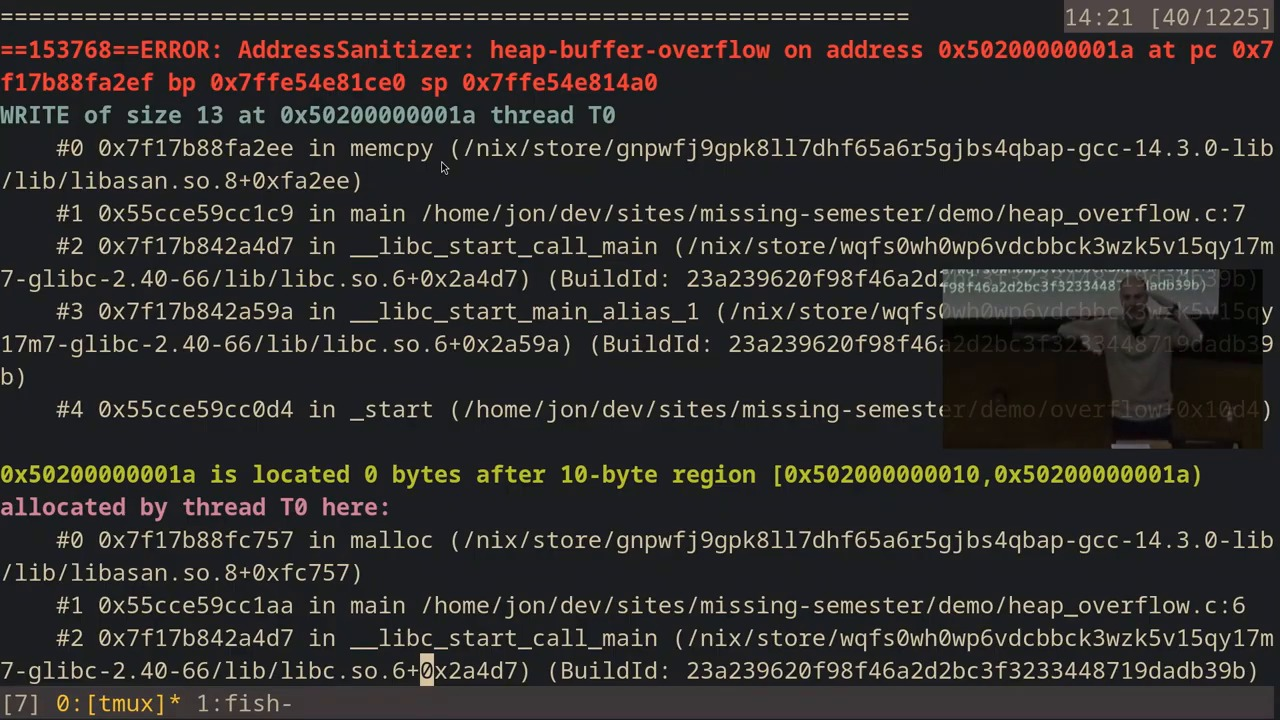
\includegraphics[width=0.92\textwidth]{figures/fig_18_asan.jpg}
\caption{AddressSanitizer 报告 heap-buffer-overflow，并给出 memcpy 所在的调用栈\vtag}
\end{figure}
\srcnote{00:49:00--00:49:15}
\end{minipage}


用 \texttt{-fsanitize=address} 编译，告诉编译器插入那些额外的检查指令。再运行，它立刻报告了问题：它所在的指令，一个回溯，就像在 rr 里看到的那样，列出出问题时的调用链，确实是 \texttt{memcpy} 在做复制。

\noindent\begin{minipage}{\textwidth}
\begin{figure}[H]
\centering
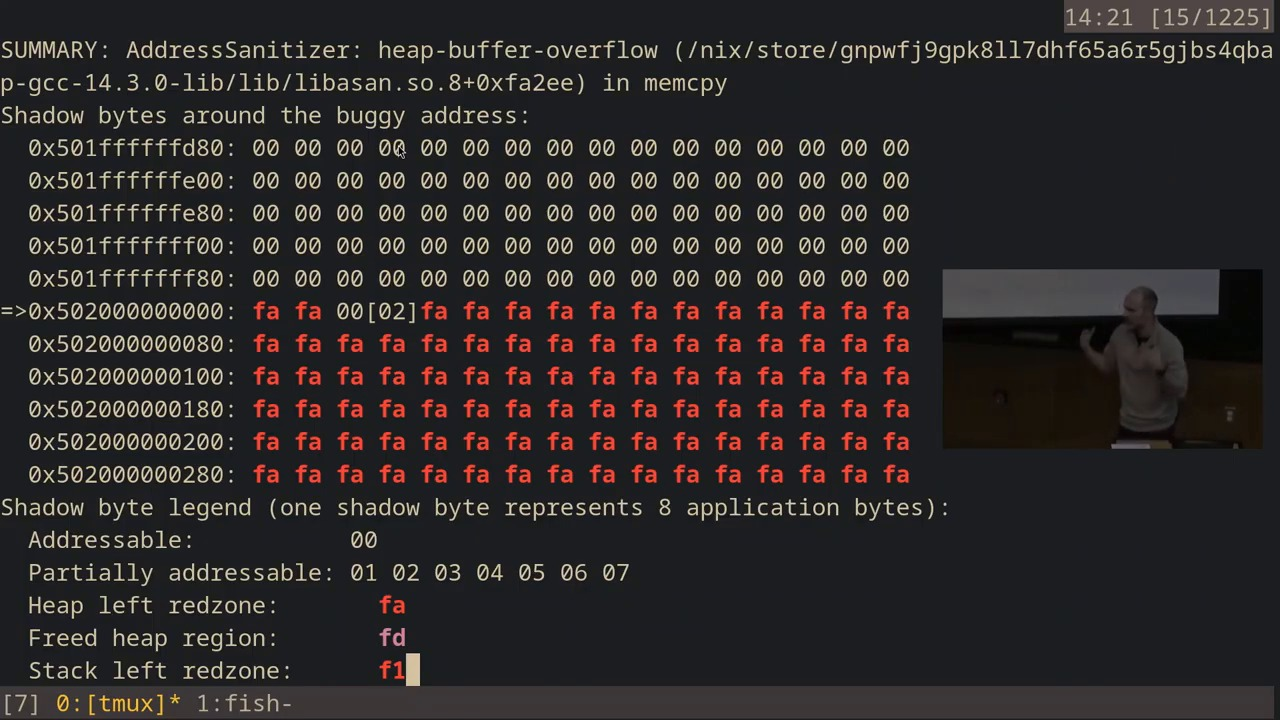
\includegraphics[width=0.92\textwidth]{figures/fig_19_asan_shadow.jpg}
\caption{影子内存图标出被越界写入的字节，下方图例解释每种标记\vtag}
\end{figure}
\srcnote{00:50:00--00:50:15}
\end{minipage}


它还给出被覆盖的内存最初在哪里分配，以及内存的内容、哪些部分被覆盖、被什么覆盖。现在你对 bug 的确切性质有了多得多的信息。

\begin{lstlisting}[language=bash]
gcc -g heap_overflow.c -o heap_overflow
./heap_overflow
gcc -g -fsanitize=address heap_overflow.c -o heap_overflow
./heap_overflow
\end{lstlisting}

讲者说，运行时更强的语言往往由运行时完成更多这类检查，有时默认关闭，因为开销可能很大；很多语言也提供绕过检查的方法，正因为它有时很昂贵，比如 Java 的 unsafe 操作允许直接操作内存，也会出现类似问题。AddressSanitizer 不能用于 Java 或 Python 程序，因为它们依赖运行时，不是原生代码，但这些语言要么语言本身支持很多检查，要么有专门工具。还有很多其他 sanitizer，比如检测程序中不同线程之间并发竞争的。如果你写很多原生程序，比如 C、C++、Objective-C、Rust，值得熟悉它们。代价是需要重新编译应用。

\begin{knowledgebox}{常见的 sanitizer}
讲义作者补充：Clang 和 GCC 提供的常用 sanitizer 包括 AddressSanitizer（\texttt{-fsanitize=address}，越界与释放后使用）、ThreadSanitizer（\texttt{-fsanitize=thread}，数据竞争）、UndefinedBehaviorSanitizer（\texttt{-fsanitize=undefined}，整数溢出等未定义行为）和 MemorySanitizer（未初始化读取，仅 Clang）。它们通常会让程序变慢数倍，适合在测试和 CI 中开启。
\end{knowledgebox}

\subsection{Valgrind}

也有不需要重新构建、直接运行原程序就能检测这类问题的工具，这在程序是别人构建的、不归你管时很有用，比如 Valgrind。讲者解释，Valgrind 是一个可扩展的程序解释器：它假装自己是 CPU，拿到你的程序并执行它的指令，因为它假装是 CPU，所以能在每条指令前后做特殊的事情。这意味着它比在 CPU 上正常运行慢得多，但能检查多得多的东西：它可以检查程序在任何地方的每一次内存操作，不需要任何插桩，从而给出非常深入的分析。它也常用于性能分析，提供精确到指令的分析信息，比如这个函数执行了多少条指令、多少个周期，因为它真的观察到了每条指令的执行；但同样会大大拖慢程序。

\subsection{用 AI 辅助调试}

讲者说，他发现 AI 对某一类调试极其有用。一类是晦涩的错误信息：通常别人已经以稍有不同的形式见过同样的错误，内存地址、程序名略有不同，这在搜索引擎里很难搜；交给 LLM，它们往往能识别出来。另一类是跨越语言边界的程序：比如一个 Python 程序链接了一个 Rust 库，后者又用了一个 C 库。如果 Python 程序里出现奇怪的行为，而根源是 C 程序的 bug，自己调试会非常痛苦。LLM 在这方面可以非常好，尤其是你让它能访问这三个依赖的源代码：告诉它“我在 Python 代码中观察到这个行为”，它会写小的复现程序，找到能复现 bug 的小用例，再追踪到“这是这个 Rust 调用”，然后到 Rust 代码中只用 Rust 复现，再意识到“这其实是这个 C 调用”，到 C 里写个 C 程序复现。

\begin{importantbox}{AI 擅长找 bug，不一定擅长修 bug}
讲者的经验是：AI 不太擅长修复这类 bug，但很擅长替你找到它们，单这一点就能节省时间。它对堆栈跟踪、崩溃跟踪也很有帮助：示例程序的调用栈很短，但如果调用栈有 100 层深，浏览起来会很烦，尤其是不熟悉的代码库，LLM 可以帮你找出真正关心的是哪个函数。
\end{importantbox}

\section{性能分析：计时与资源监控}

\subsection{time}

\noindent\begin{minipage}{\textwidth}
\begin{figure}[H]
\centering
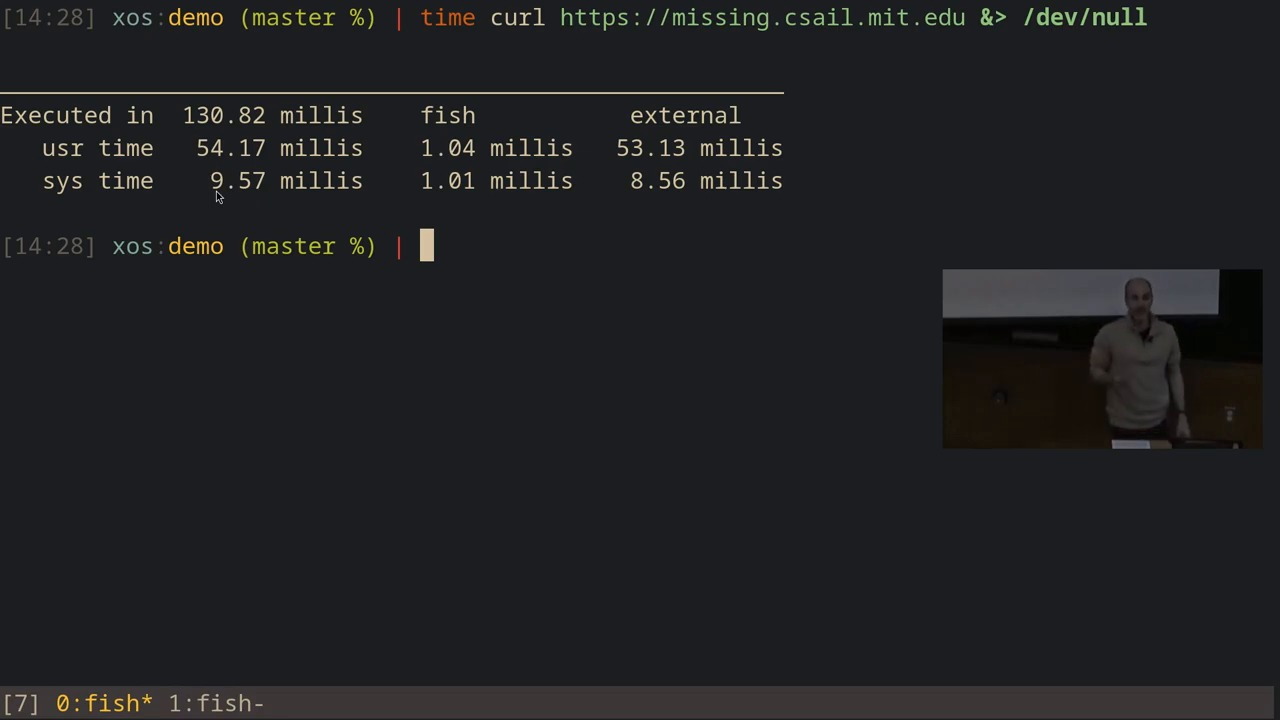
\includegraphics[width=0.92\textwidth]{figures/fig_20_time_curl.jpg}
\caption{\texttt{time curl} 显示墙钟时间约 130 毫秒，而用户态时间只有约 54 毫秒\vtag}
\end{figure}
\srcnote{00:56:30--00:56:45}
\end{minipage}


讲者说，虽然时间不多了，还是要进入性能分析。性能分析和调试出奇地相关：如果能理解程序在做什么，通常也能用来理解它的性能。首先是计时：怎样测量一件事花了多久？几乎每个 Shell 里都有 \texttt{time}，它内置在 Shell 中，后面跟任何想执行的命令，运行后给出一个摘要，不同 Shell 略有不同，但信息相同，通常有三个数：real、user 和 sys。real 是流逝的墙钟时间，就是从按下回车到输出结束，看钟表过去了多久；user 是 CPU 花在你的代码上的时间；sys 是 CPU 在内核中为这个程序执行的时间。

之所以说 CPU 时间，是因为假如有 10 个 CPU，过了 1 秒，10 个 CPU 都工作了 1 秒，那就过去了 10 个 CPU 秒，尽管实际只过了 1 秒。在这个例子里，实际执行花了 130 毫秒，但 CPU 时间只有 54 毫秒，内核时间只有 9 毫秒，其余时间去哪了？都花在等待上。\texttt{curl} 通过 HTTP 访问远程服务器，这里是获取课程网站，大量时间花在等待数据包到达另一端的服务器再返回，墙钟时间流逝了，却没有花 CPU 时间。

\subsection{hyperfine}

\noindent\begin{minipage}{\textwidth}
\begin{figure}[H]
\centering
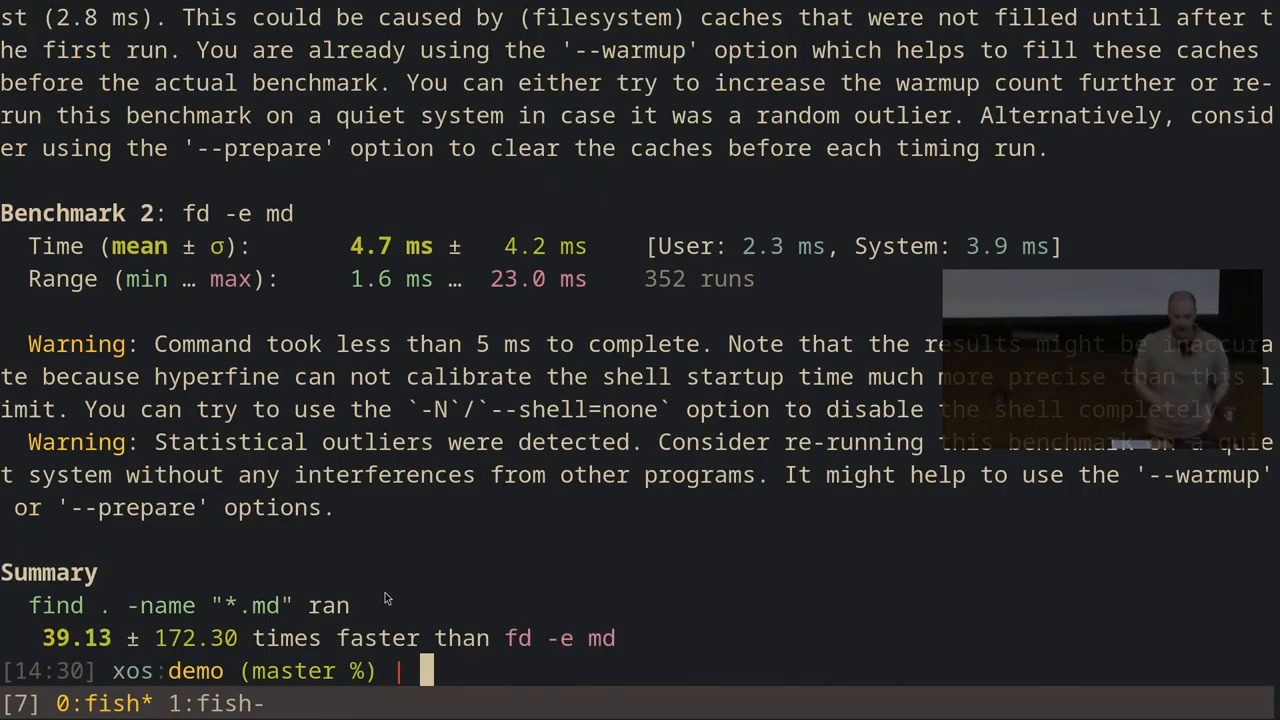
\includegraphics[width=0.92\textwidth]{figures/fig_21_hyperfine.jpg}
\caption{hyperfine 多次运行 find 与 fd 并给出带标准差的对比结果\vtag}
\end{figure}
\srcnote{00:58:00--00:58:15}
\end{minipage}


用 \texttt{time} 分别运行两个程序，也是比较它们最简单的方式之一。这可行但不太可靠，因为多次运行同一个程序，时间会有所波动：这次 124，那次 138；这次内核里花了 20 毫秒，之前只花了 9 毫秒。哪个才是真的？有人为此写了工具，比如 \texttt{hyperfine}：给它任意数量的命令，它把每个都运行多次，测量执行时间，用统计方法算出两个程序加速比的标准差等。讲者比较了 \texttt{find} 和改进版的 \texttt{fd}，结果说 \texttt{find} 比 \texttt{fd} 快了大约 40 倍。他说这是一个很特殊的情况：在一个几乎为空的目录里，\texttt{fd} 并没有针对这种情况优化；但它确实给出了统计上的信心，说明这不只是碰巧运行了一次的结果。

\begin{lstlisting}[language=bash]
time curl https://missing.csail.mit.edu > /dev/null
hyperfine --warmup 3 'fd -e jpg' 'find . -iname "*.jpg"'
\end{lstlisting}

\subsection{监控资源使用}

\noindent\begin{minipage}{\textwidth}
\begin{figure}[H]
\centering
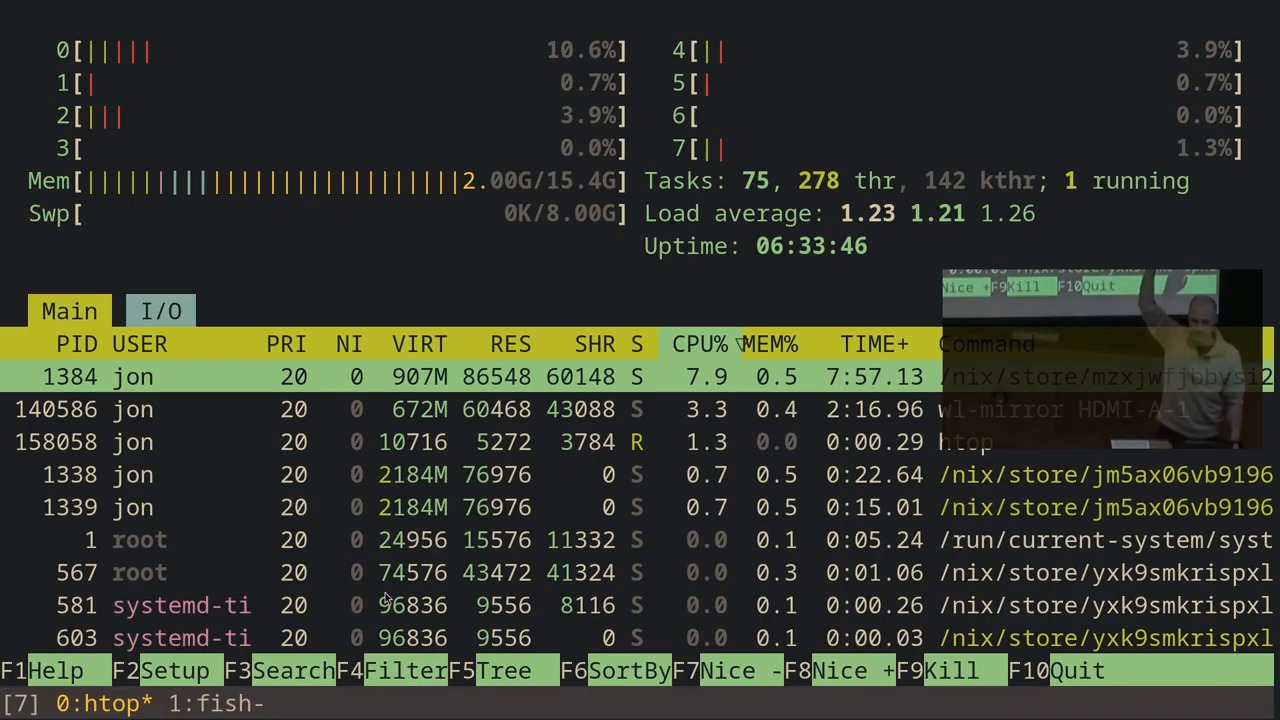
\includegraphics[width=0.92\textwidth]{figures/fig_22_htop.jpg}
\caption{htop 显示每个核心的利用率、内存、平均负载和进程列表\vtag}
\end{figure}
\srcnote{00:59:00--00:59:15}
\end{minipage}


讲者说，做性能分析时，有时仅仅了解系统在做什么就很有用。程序很慢：是因为它用满了所有 CPU 核心？还是只用了一个核心？还是磁盘慢？监控资源使用非常有价值。\texttt{htop} 显示他有八个核心，以及每个核心的 CPU 利用率、内存使用情况，右边是平均负载（load average），他建议大家去查查这几个数的含义：大致是过去一段时间里需要多少个 CPU 核心，三个数对应越来越长的时间窗口，可以看出负载随时间的变化。底部是当前系统上运行的所有进程，可以切换视图、按不同列排序、浏览以了解更多。

\noindent\begin{minipage}{\textwidth}
\begin{figure}[H]
\centering
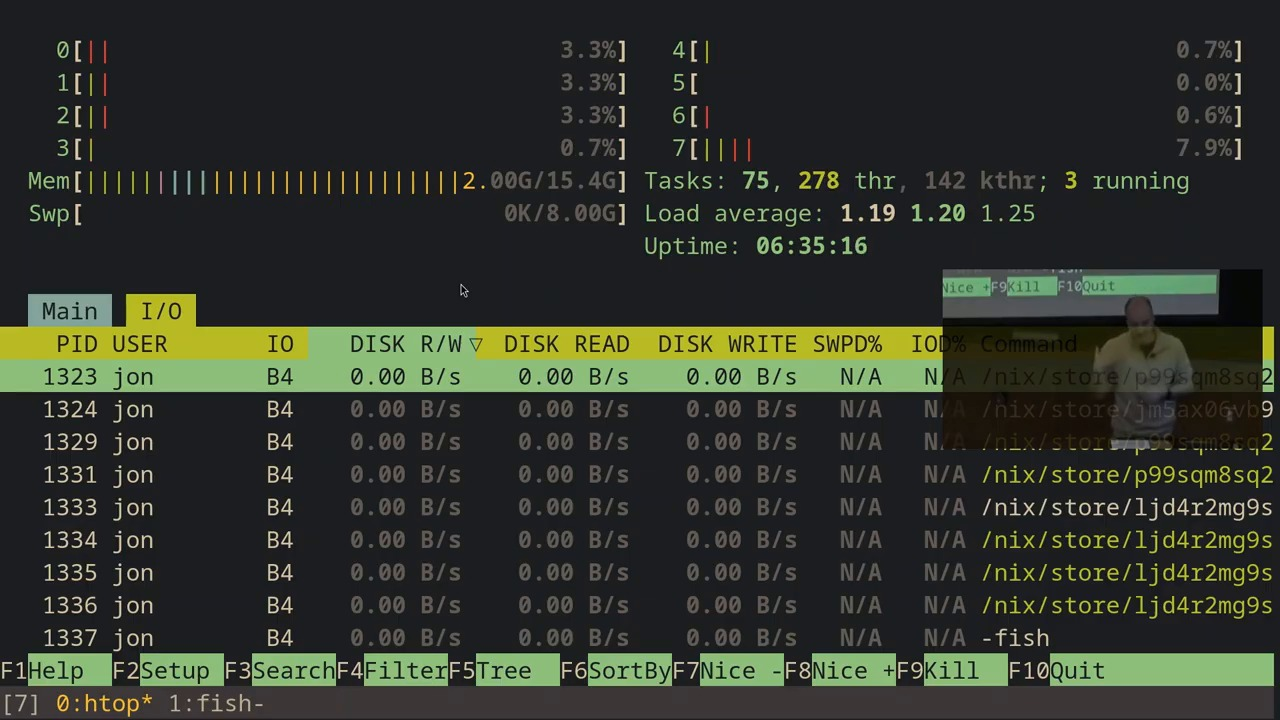
\includegraphics[width=0.92\textwidth]{figures/fig_23_htop_io.jpg}
\caption{htop 的 I/O 标签页显示每个进程的磁盘读写情况\vtag}
\end{figure}
\srcnote{01:00:30--01:00:45}
\end{minipage}


还可以切换到其他标签页，比如 I/O 标签页显示每个进程的磁盘读写和网络读写，可以按这些排序，看出系统资源都用到了哪里，从而推断程序的瓶颈。还有很多专门工具：\texttt{iotop} 专门显示输入输出的详细信息；\texttt{free} 显示内存使用；\texttt{lsof} 显示当前打开的文件；\texttt{ss} 显示网络连接，比如哪些端口开着、哪些连接连到了哪里。\texttt{btop} 是比 \texttt{htop} 更好的版本，显示大量系统统计，可以配置成只显示你关心的东西。

\begin{knowledgebox}{平均负载怎么读}
讲义作者补充：Linux 的三个平均负载分别是过去 1、5、15 分钟内处于可运行（以及不可中断等待）状态的平均任务数。在 8 核机器上，负载 1.2 表示平均只需要大约 1.2 个核心；如果负载长期高于核心数，说明任务在排队等待 CPU 或 I/O。
\end{knowledgebox}

\section{性能分析：perf 与火焰图}

\subsection{采样分析器 perf}

\noindent\begin{minipage}{\textwidth}
\begin{figure}[H]
\centering
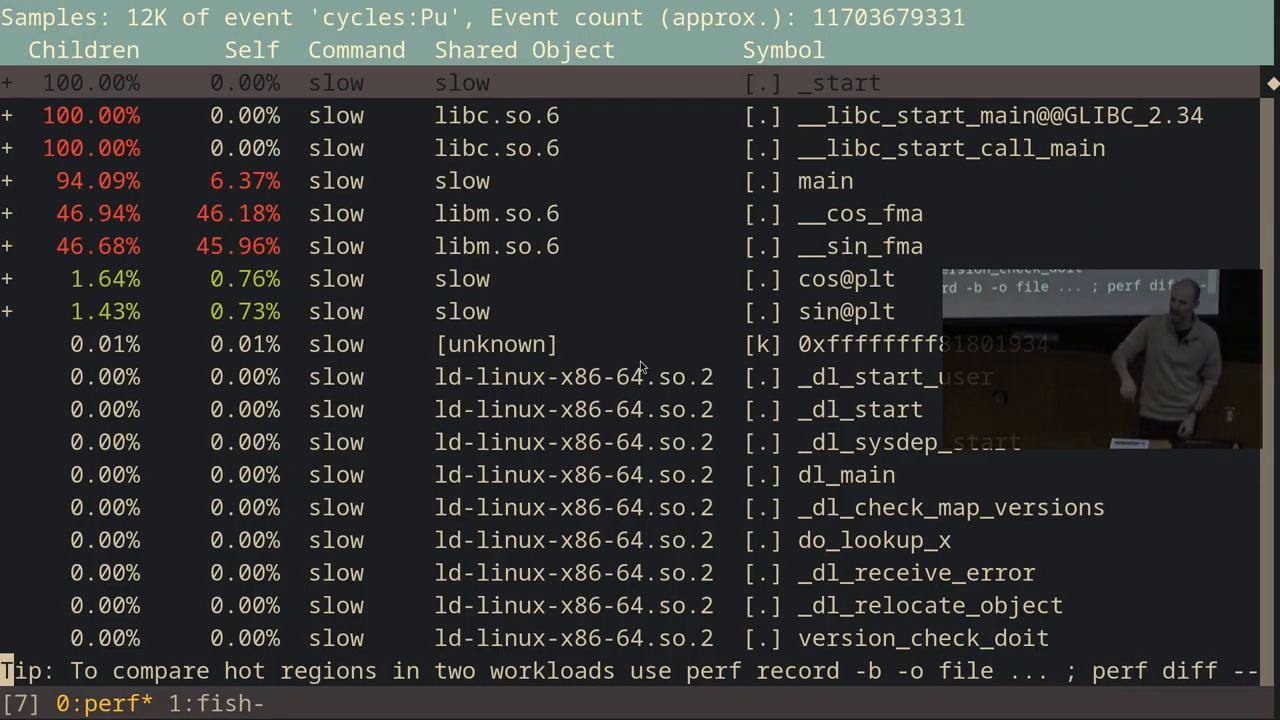
\includegraphics[width=0.92\textwidth]{figures/fig_24_perf_report.jpg}
\caption{perf report：Children 列包含子函数，Self 列中 cos 和 sin 各占约 43\%\vtag}
\end{figure}
\srcnote{01:03:00--01:03:15}
\end{minipage}


讲者说，真正到了“我要让这个程序更快”的阶段，你需要记录某个程序的信息，找出它最热的部分，即程序把时间花在哪里，深入到函数内部，这就要用 \texttt{perf}。他编译了一个 \texttt{slow.c}，它做一些数学运算，运行一会儿后退出，算出某个结果。用 \texttt{perf record -g} 运行程序，\texttt{-g} 表示捕获调用图信息。\texttt{perf} 是一个采样分析器（sampling profiler）：每隔一段时间暂停程序，查看每个 CPU 正在执行程序的哪里，记录下来，再让它继续运行，每秒很多次，从而得到 CPU 在程序哪里花时间最多的样本。

完成后运行 \texttt{perf report}，它显示：100\% 的时间花在 \texttt{\_start} 中或其下。第一列 Children 是这个函数及其子函数，即它调用的一切，显然 \texttt{\_start} 是二进制的起点，所有时间都在它下面；第二列是只花在这个函数本身、不含后代的时间：有 43.6 个百分点花在计算余弦上，约 43\% 花在计算正弦上。

\noindent\begin{minipage}{\textwidth}
\begin{figure}[H]
\centering
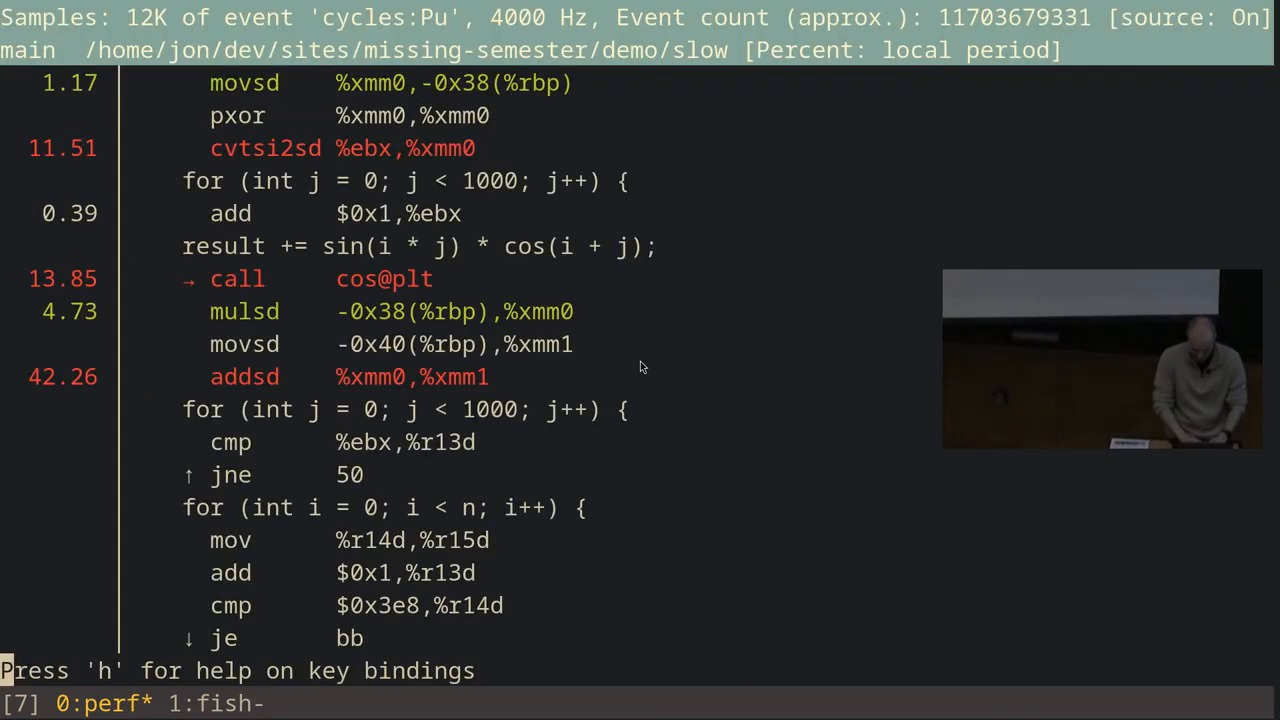
\includegraphics[width=0.92\textwidth]{figures/fig_25_perf_annotate.jpg}
\caption{annotate 视图把 C 源码行与汇编指令交错显示，并标出各自的耗时百分比\vtag}
\end{figure}
\srcnote{01:04:00--01:04:15}
\end{minipage}


还可以查看带注释的代码清单，这里用原始汇编注释这个函数。按 \texttt{h} 可以得到帮助信息，可以显示行号、源代码行等。讲者对 \texttt{main} 做了注释，打开源代码视图后，可以看到这个 for 循环对应这条指令，C 代码和汇编指令交错显示，每行汇编所占总计算时间的百分比也标了出来，于是可以深入到“我的这行代码的这一部分是 CPU 花时间最多的地方”。

\begin{lstlisting}[language=bash]
gcc -g -O2 slow.c -o slow -lm
perf record -g ./slow
perf report
perf script | inferno-collapse-perf | inferno-flamegraph > slow.svg
\end{lstlisting}

\subsection{火焰图}

\noindent\begin{minipage}{\textwidth}
\begin{figure}[H]
\centering
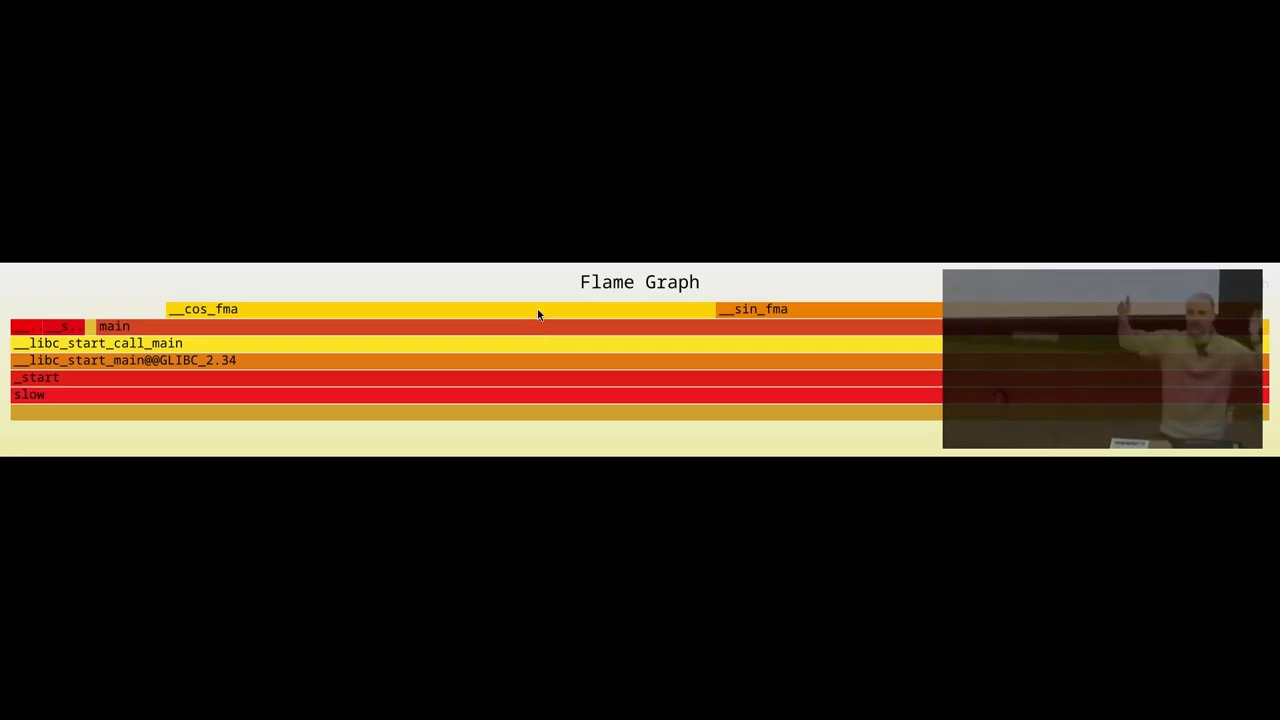
\includegraphics[width=0.92\textwidth]{figures/fig_26_flamegraph.jpg}
\caption{slow 程序的火焰图：main 之上 cos 与 sin 大约各占一半宽度\vtag}
\end{figure}
\srcnote{01:05:30--01:05:45}
\end{minipage}


讲者说，这些信息可能难以解析，人类不太擅长解析这类信息，尤其是大规模的，于是有人做了更好的可视化工具，比如火焰图（flame graph）。他用的是 Inferno，火焰图的 Rust 移植版，只是因为碰巧装了它：把 \texttt{perf script} 的输出交给几个脚本处理，生成一个 SVG 文件。打开它，最底部是二进制的入口，往上一点是 \texttt{main} 函数；在 \texttt{main} 中，条的宽度表示花在那里的时间，可以看到 \texttt{main} 大约一半时间在余弦、一半在正弦。因为着色方式，它看起来像一大片火焰，越宽的火焰就是花时间越多的地方。讲义里有一个更复杂程序的例子；在浏览器里打开时还可以点击，点击放大、展开不同帧的信息等。

\begin{warningbox}{采样带来的不精确}
讲者提醒，\texttt{perf} 是采样分析器，只能看到它中断程序时 CPU 在哪里，所以信息不完美。可以提高采样频率，但程序也会因为更频繁地暂停而变慢。想要非常精确的信息，可以用 Valgrind 运行：它像 CPU 一样解释每一条汇编指令，不是采样而是真正追踪，能测量每条汇编指令被调用了多少次，但因此往往相当慢。Valgrind 有很多不同模式（插件），比如检查内存使用是否正确，或者统计每条指令被调用的次数。
\end{warningbox}

\begin{practicebox}{给自己的程序画火焰图}
讲义作者整理：按课程讲义保存 \texttt{slow.c}，用 \texttt{perf record -g ./slow} 采样，再用 \texttt{perf report} 找出 Self 列最大的函数；然后生成火焰图，在浏览器中打开并点击放大；最后尝试修改代码（例如把重复计算移出循环），重新采样比较火焰图的变化。没有 Linux 时可以用 Speedscope 等工具查看采样结果。
\end{practicebox}

\subsection{可视化性能数据}

讲者最后说，性能分析不只是评估程序各部分运行得多快，还包括查看程序的输出、理解它为什么那样表现，以及程序行为如何随输入变化。比如 \texttt{grep} 这样的工具，你可能想了解它的速度怎样随输入大小、模式长度或模式复杂度变化。这时需要可视化数据：一大堆“用这个输入大小、这个模式大小，花了这么多微秒”的文本，像一张长长的 Excel 表，不会有多大用处。

终端里有一些便于快速绘图的工具，比如 gnuplot，它是为 Shell 设计的：和 \texttt{bpftrace} 一样可以用 \texttt{-e} 传入一个小小的绘图语言，比如把标准输入的这一列对那一列画成 x 对 y，还可以改颜色、画多条线、改坐标轴。要做更深入的分析，可以用 Python 的 matplotlib，或者 R 的 ggplot2。讲者特别喜欢 ggplot2 的分面（facet wrap）功能：比如 x 轴是输入大小，y 轴是 \texttt{grep} 的执行时间，颜色对应模式长度，再按模式复杂度每种画一张图并排放在一起比较，甚至排成网格，让另外的列沿横向和纵向递增。这样可以把五维的数据画成肉眼能看懂的图。讲者说，这是性能分析的超能力之一：不仅提取程序行为的信息，还把它可视化，从而发现问题或奇怪的模式。

\begin{importantbox}{回到日志}
讲者以呼应开头作结：当你想做性能分析时，需要的往往是输入有多大、某个函数花了多久、某个内部图结构有多大这类信息。如果早早想清楚记录什么、怎样记录，尽量使用便于事后解析（比如用于绘图）的结构化日志，并主动记录各种规模信息，那么以后要分析程序时，日志里就已经有了绘制这些图所需的全部信息，可以指出程序中潜在的问题或“规模悬崖”。
\end{importantbox}

\section{总结}

\begin{itemize}
\item 打印调试简单有效；把有用的打印改成带级别的结构化日志，下次就不必从头开始。
\item 调试器（GDB、LLDB、PDB）让你设断点、单步、查看状态和设置监视点；rr 记录执行后可以反向执行，适合偶发与难复现的 bug，但要警惕海森堡 bug。
\item strace 追踪系统调用，\texttt{-f} 跟踪子进程，\texttt{-e} 过滤；bpftrace 借助 eBPF 在内核中运行小程序，biolatency、opensnoop 等现成工具建立在它之上；tcpdump 和 Wireshark 用于网络调试。
\item AddressSanitizer 等 sanitizer 在编译时插入检查，Valgrind 无需重新编译就能逐条指令检查，但很慢。
\item AI 擅长解读晦涩错误、跨语言定位 bug 和浏览长调用栈。
\item 性能分析从 \texttt{time}、hyperfine 和 htop 开始，用 perf 找热点，用火焰图可视化，用 gnuplot、matplotlib、ggplot2 观察性能如何随输入变化。
\end{itemize}

\begin{practicebox}{自测}
\begin{enumerate}
\item 为什么 \texttt{time} 报告的 real 可能远大于 user 加 sys？反过来什么时候 user 会大于 real？
\item 用 rr 定位 \texttt{corruption.c} 的 bug 时，watch 加 reverse-continue 相比反复设断点重跑省掉了什么？
\item 一个进程看起来卡住了，用 \texttt{strace -p} 附加后没有任何输出，这说明什么？
\item AddressSanitizer 与 Valgrind 都能发现越界写入，二者在使用条件和开销上有何不同？
\item 在火焰图中，一个很宽但上方没有子帧的函数意味着什么？
\end{enumerate}
\end{practicebox}

\end{document}
